%% Bemærk:
%%          Resten af rapporten følger en stil hvor indledninger skrives
%%          med \sffamlily-typen. Denne stil bør også følges her.
%%
{
{\sffamily
I dette kapitel vil vi afprøve vores to metoder, på fabrikeret test
billeder og på malerier fra vores billedet database og se hvordan
metoderne virker. Udover det, vil vi finde tærskelværdier til
kantdetektion, floodfill, margin, regioners masse og regioners størrelse
samt sløring, ud fra observationer gjort under afprøvning. Vi vil også
afprøve den generelle udtrækning af regioner og kommer ind på dens
fordele og ulemper.}

\section{Tærskelværdier\label{terskelverdi}}
I vores program er der 3 forskellige tærskelværdier som påvirker hvordan
metoden analysere billedet. Marginens brede, afvigelsen af farven i
floodfill og afvigelsen i farven i kandtdetectionen. Alle 3 tærskelværdier er
blevet introduceret i deres respektive afsnit, men ingen konkrate tal
er opgivet. I dette afsnit vil vi opgive de tal, samt en forklaring på
hvorfor vi har valt lige de tal.

\subsection{Marginens brede}
Vi regner marginens brede, $MB$ ud fra en procent af billedets brede og
højde. I afsnittet \ref{opdeling_af_billeder.tex} kom vi frem til en
usikkerhed på $2.1 \%$. Så vores $MB$ skal mindst
være på $2.1 \%$. Ud over det er den minimale forskel på 2 snit vi foretager os,
forskellen mellem det gyldne snit og $\frac{2}{3}$, som vi udregnet i
sektion \ref{opdeling_af_billeder.tex} til maksimalt at have en $MB$ på
$2.43$, for at margin ikke krydser. Så $MB \in [2.1, 2.43]$. Vi har valt
at sætte $MB = 2.4$, da vi derved kan tage højde for uforresette
usikkerhed. XXX(er det en dog nok forklaring).

\subsection{Afvigelsen af farver i kandtdetection}
Det vi bruger kandtdetection til, er af finde en kanter rundt om de
regioner som vi mener er interessante, og undgå de kanter som ligger
inde i regioner. Begge de 2 mål kan ikke altid opfyldes, men vi kan
komme så tæt på et krompromi mellem en perfekt kant rund om region og
ingen kanter inde i region som mulige. Dette gøres ved at ændre 2
tærskelværdier i kantdetectionen ud for observationer som vi har taget
på billederne i forvejen. Vi har valt at dele billederne som vi
observere op i 9 kategorier, som kan ses i tabel
\ref{thressholdsTabelKant}, Kategorier er en grove opdeling af
billederne efter detaljer og farve intensitet, som bruges til at give en
bedre indblik på billedets opbygning. 

\subsubsection{Sammenligninger}
Vi har set på XX(hvor mange) antal malerier og har fundet de
tærskelværdier som vi mener passer bæst på billedet. Vi vil illustrerer
den fremgange måden vi har brugt til at finde tærskelværdierne på, på
maleriet \ref{kDetalier}. Maleriet er malet med mange farver og med
masser af detaljer. Vi ser først på tærskelværdierne
$[0,0],[100,100]......[900,900],[1000,1000]$ se figur \ref{allesammen1}
og \ref{allesammen2}, og finde det interval hvor malerriet ikke har
mistet nogle af kanterne rundt om regionerne i nu, men vil det, i næste
interval. I illustration vurdere vi det til billedet \ref{300-300}, da
billedet \ref{400-400} har mistet for mange af de kanter, som vi gerne
vil beholde. Så tærskelværdien som vi gerne vil finde frem til, befinder
sig fra $[300,300]$ og frem. Ved at sætte den anden tærskelværdig op
lidt af gangen kan vi igen få en række billeder at vælge imellem, for at
få det beste resultat, se sammenligningen i figur \ref{allesammen3}. som
man kan se begynder det er være svær at skelne figurene i \ref{300-850}
og der er lidt for mange kanter i \ref{300-700}, så vi har valt at bruge
tærskeværdigerne $[300,750]$ for dette billedet. Man kunne god gå længer
ned og se om tærskeværdig $[300,745]$ passet bedre, men vi har valt at
holde . Det maleri vi lige har brugt er ikke særlige repræsentativ for
helle vores maleri database, så vi har taget en række billeder og brugt
samme metode på dem og kommer frem til en middel tærskelværdi, jeg viser
her en lille udsnit af dem, se figur \ref{en}, \ref{to} og \ref{tre}.

\begin{figure}[p]
    \centering
    \subfloat[100,100]{
        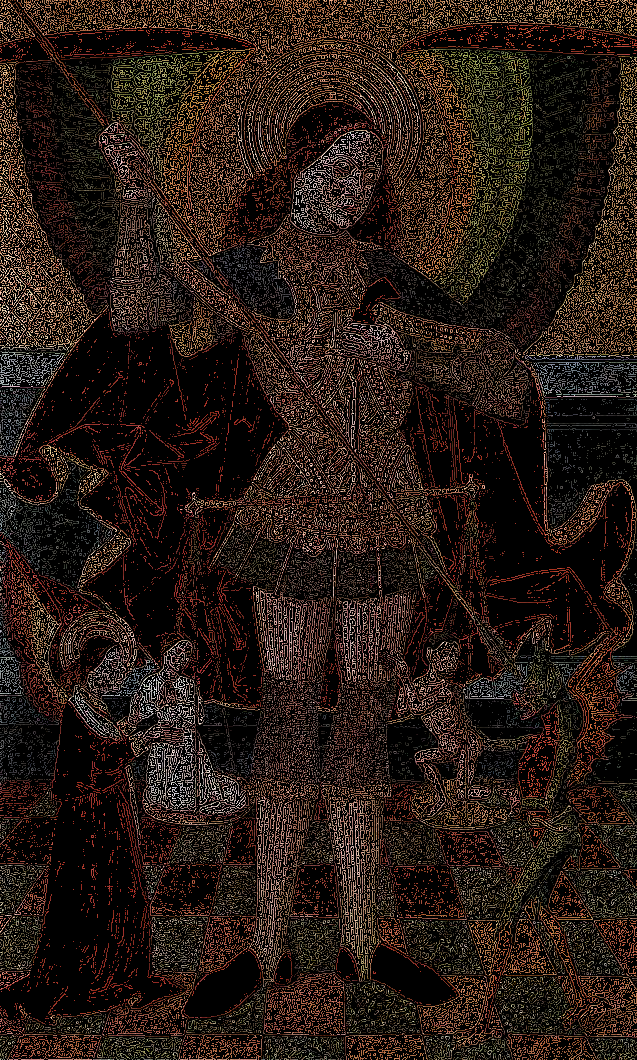
\includegraphics[angle=0,width=0.45\textwidth]{afsnit/afprovning/billeder/thressholds/krafitige_farver/krafite_detalier/1_iteration/100-100.png}
        \label{100-100}}\hspace{1em}
    \subfloat[200,200]{
        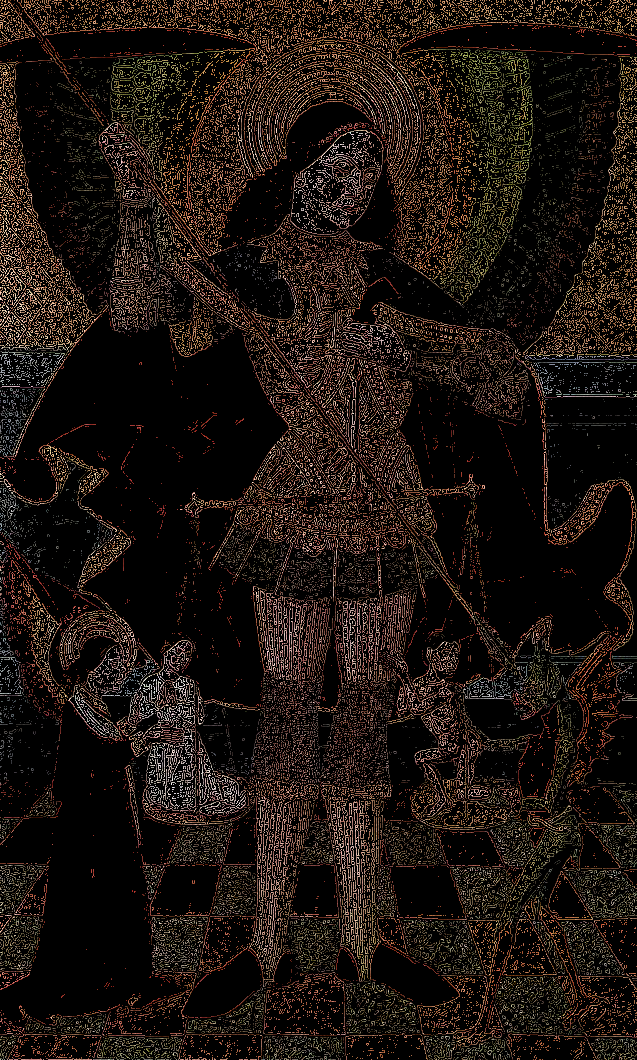
\includegraphics[angle=0,width=0.45\textwidth]{afsnit/afprovning/billeder/thressholds/krafitige_farver/krafite_detalier/1_iteration/200-200.png}
        \label{200-200}}\\
    \subfloat[300,300]{
        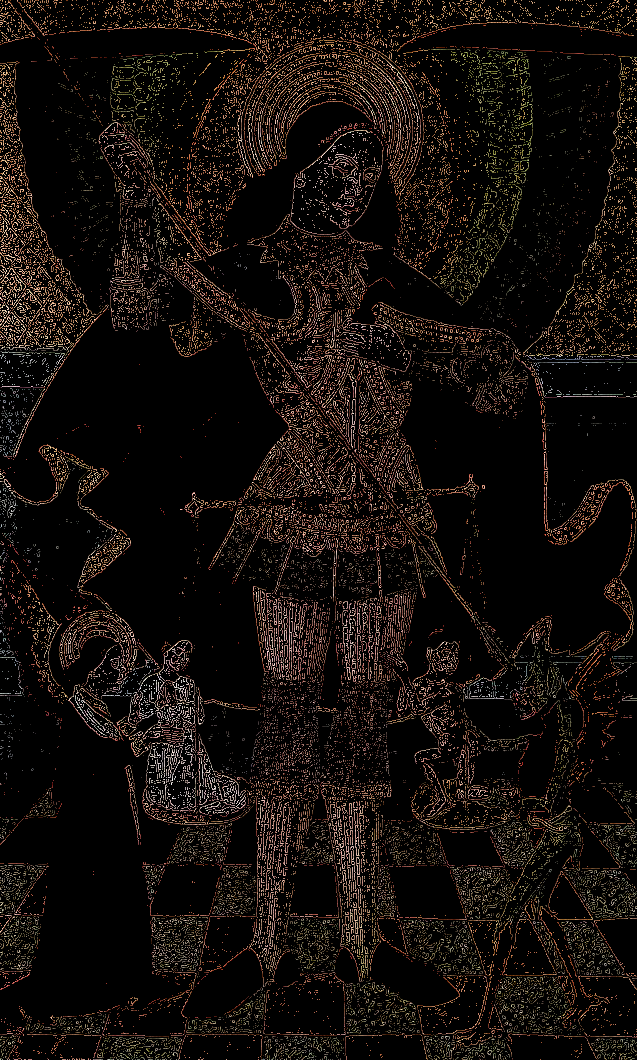
\includegraphics[angle=0,width=0.45\textwidth]{afsnit/afprovning/billeder/thressholds/krafitige_farver/krafite_detalier/1_iteration/300-300.png}
        \label{300-300}}\hspace{1em}
    \subfloat[400,400]{
        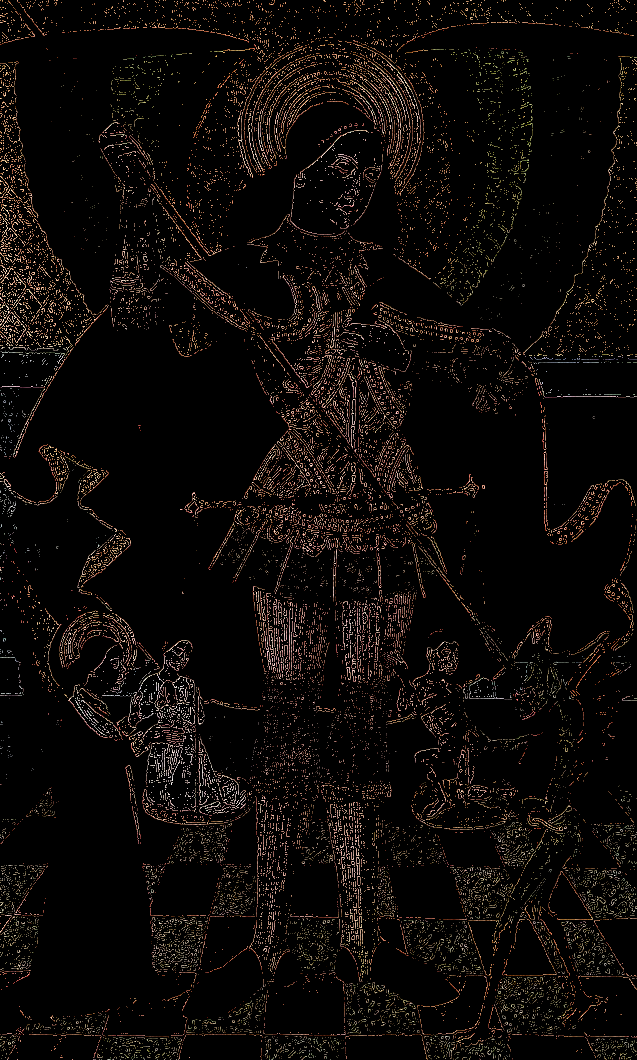
\includegraphics[angle=0,width=0.45\textwidth]{afsnit/afprovning/billeder/thressholds/krafitige_farver/krafite_detalier/1_iteration/400-400.png}
        \label{400-400}}
    \label{allesammen1}
    \caption{Hvad er et her?}
\end{figure}

\clearpage

\begin{figure}[!h]
	\centering
	\subfloat[500,500]{
        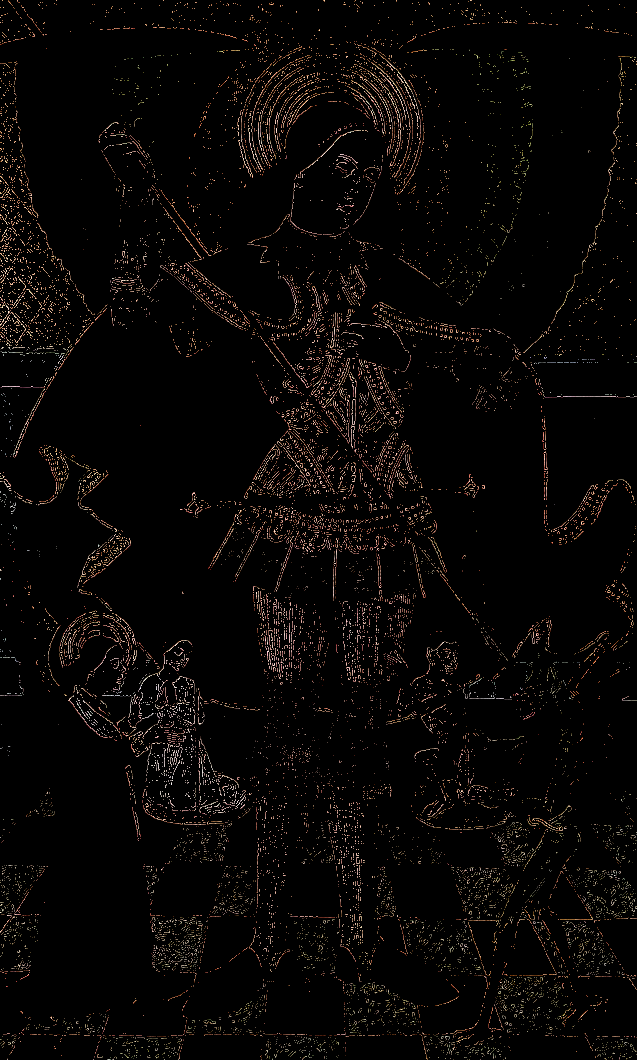
\includegraphics[angle=0,width=0.45\textwidth]{afsnit/afprovning/billeder/thressholds/krafitige_farver/krafite_detalier/1_iteration/500-500.png}
        \label{500-500}}\hspace{1em}
    \subfloat[600,600]{
        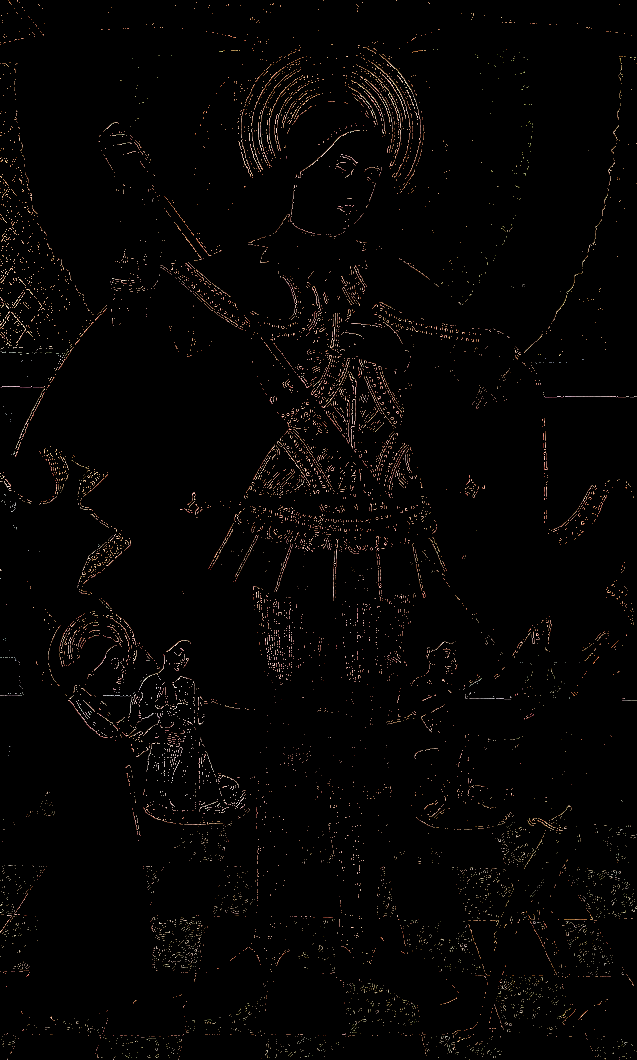
\includegraphics[angle=0,width=0.45\textwidth]{afsnit/afprovning/billeder/thressholds/krafitige_farver/krafite_detalier/1_iteration/600-600.png}
        \label{600-600}}\\
    \subfloat[700,700]{
        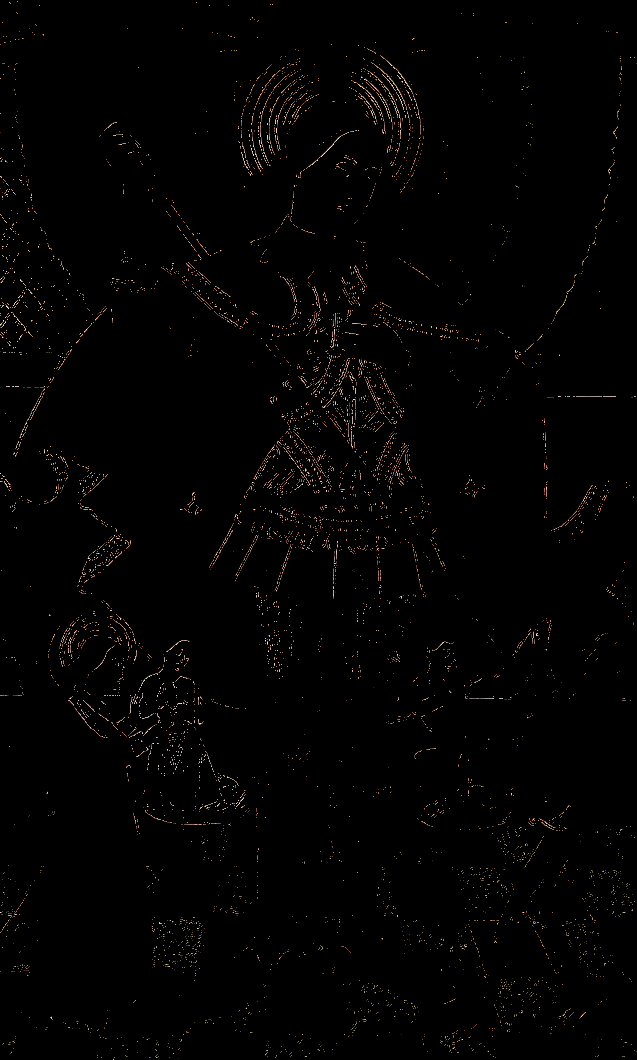
\includegraphics[angle=0,width=0.45\textwidth]{afsnit/afprovning/billeder/thressholds/krafitige_farver/krafite_detalier/1_iteration/700-700.png}
        \label{700-700}}\hspace{1em}
    \subfloat[Original]{
        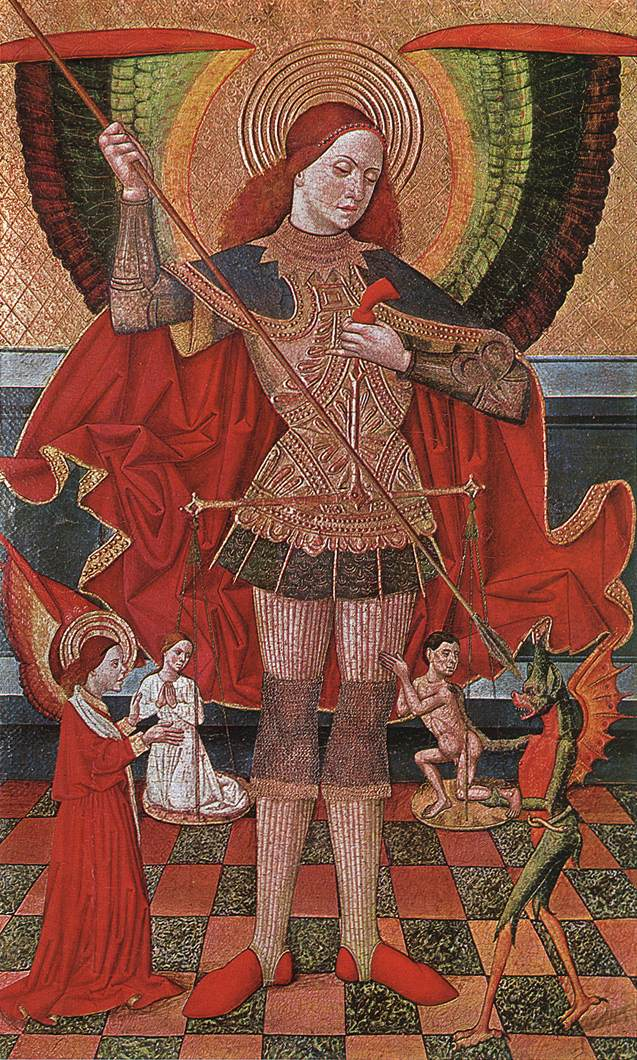
\includegraphics[angle=0,width=0.45\textwidth]{afsnit/afprovning/billeder/thressholds/krafitige_farver/krafite_detalier/kDetalier.jpg}
        \label{kDetalier}}
    \caption[]{Edgedetection på maleriet \ref{kDetalier} som har mange detaliger og kraftige farver, med tærskelværdierne fra 100-100 til 700-700}
     \label{allesammen2}
\end{figure}

\begin{figure}[!h]
    \centering
    \subfloat[300,700]{
        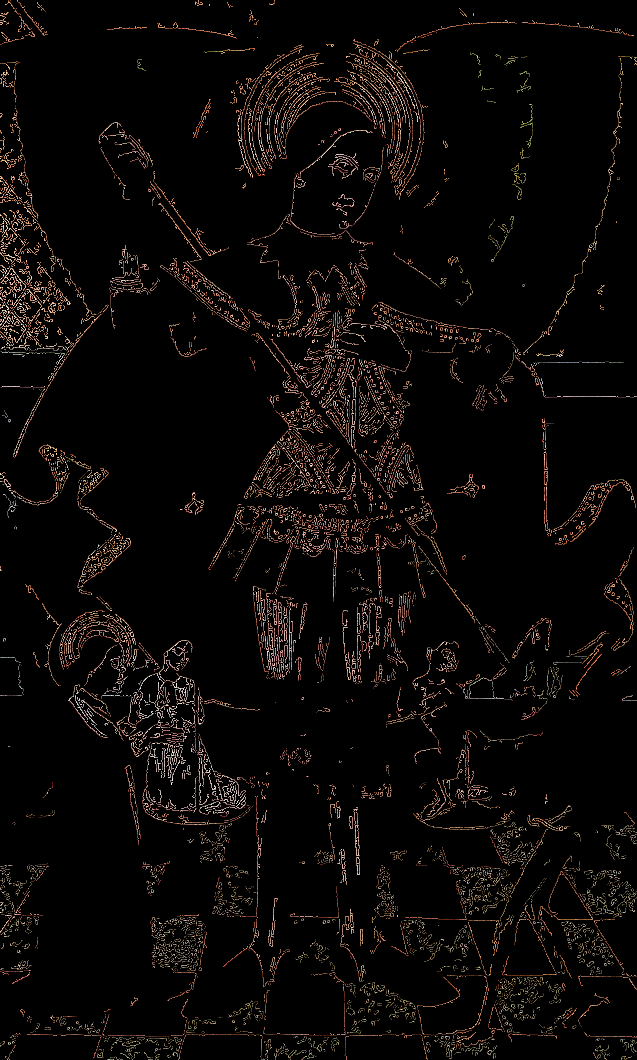
\includegraphics[angle=0,width=0.45\textwidth]{afsnit/afprovning/billeder/thressholds/krafitige_farver/krafite_detalier/2_iteration/300-700.png}
        \label{300-700}}\hspace{1em}
    \subfloat[300,750]{
        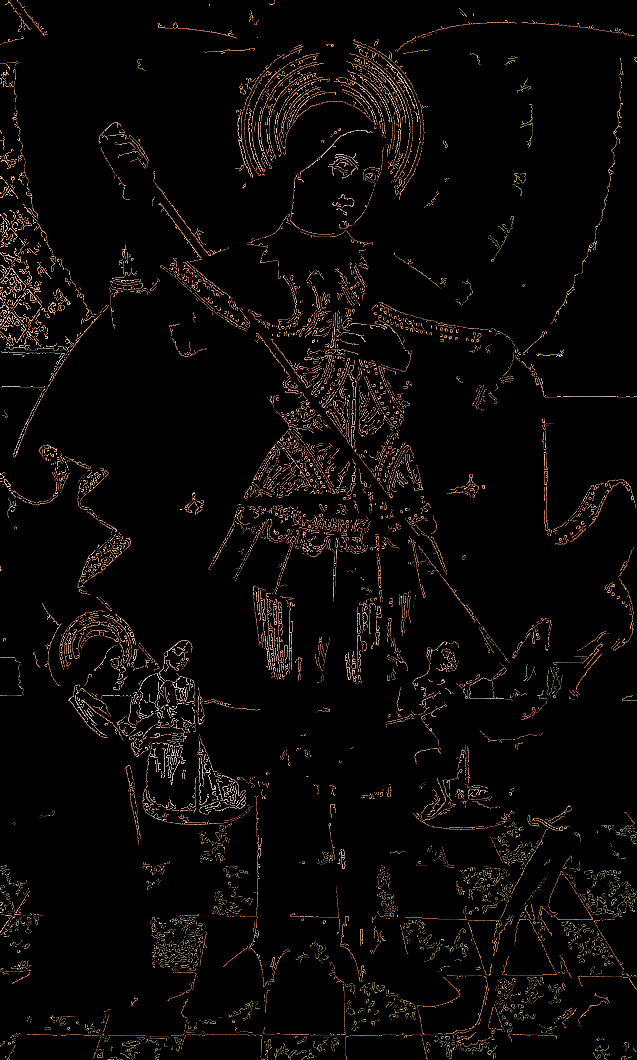
\includegraphics[angle=0,width=0.45\textwidth]{afsnit/afprovning/billeder/thressholds/krafitige_farver/krafite_detalier/2_iteration/300-750.png}
        \label{300-750}}\\
    \subfloat[300,800]{
        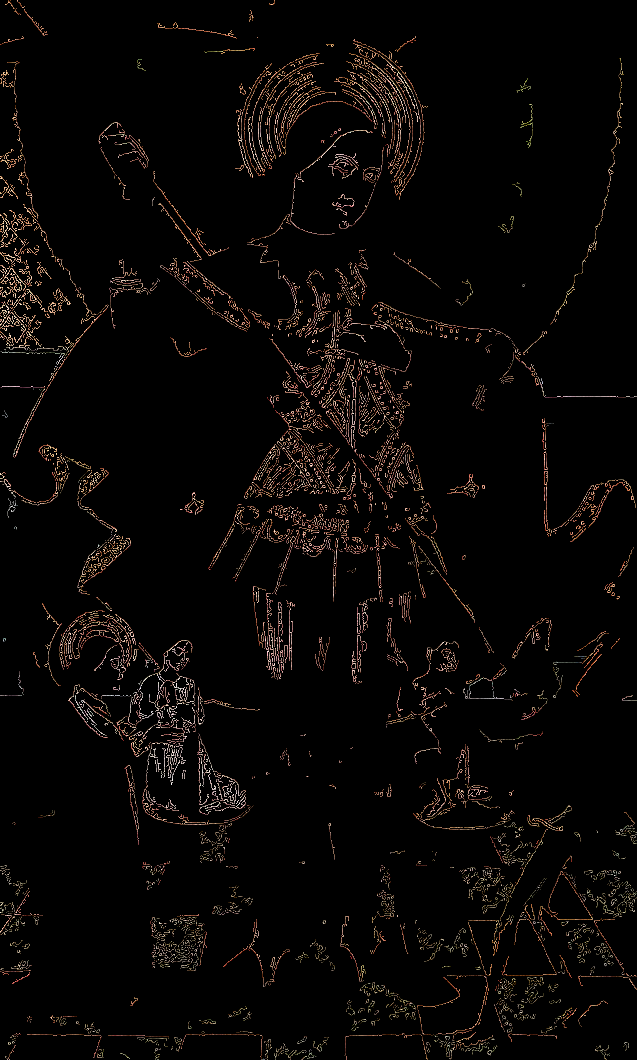
\includegraphics[angle=0,width=0.45\textwidth]{afsnit/afprovning/billeder/thressholds/krafitige_farver/krafite_detalier/2_iteration/300-800.png}
        \label{300-800}}\hspace{1em}
    \subfloat[300,850]{
        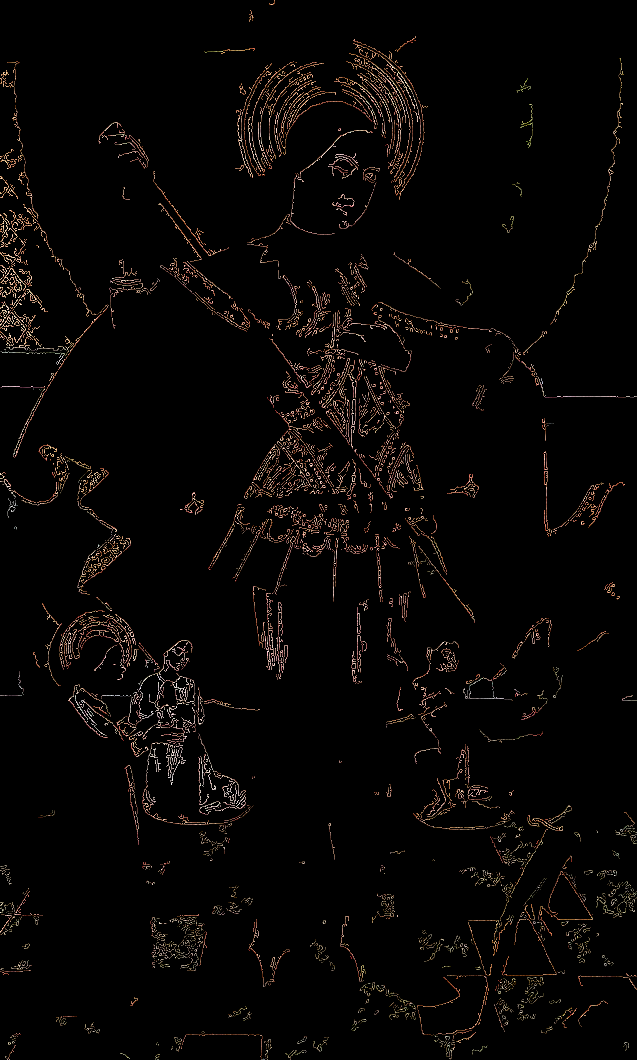
\includegraphics[angle=0,width=0.45\textwidth]{afsnit/afprovning/billeder/thressholds/krafitige_farver/krafite_detalier/2_iteration/300-850.png}
        \label{300-850}}
        \caption[]{Edgedetection hvor de 4 billeder som er intrasante taget med}
     \label{allesammen3}
\end{figure}
 
\begin{figure}[!h]
    \centering
    \subfloat[100,250]{
        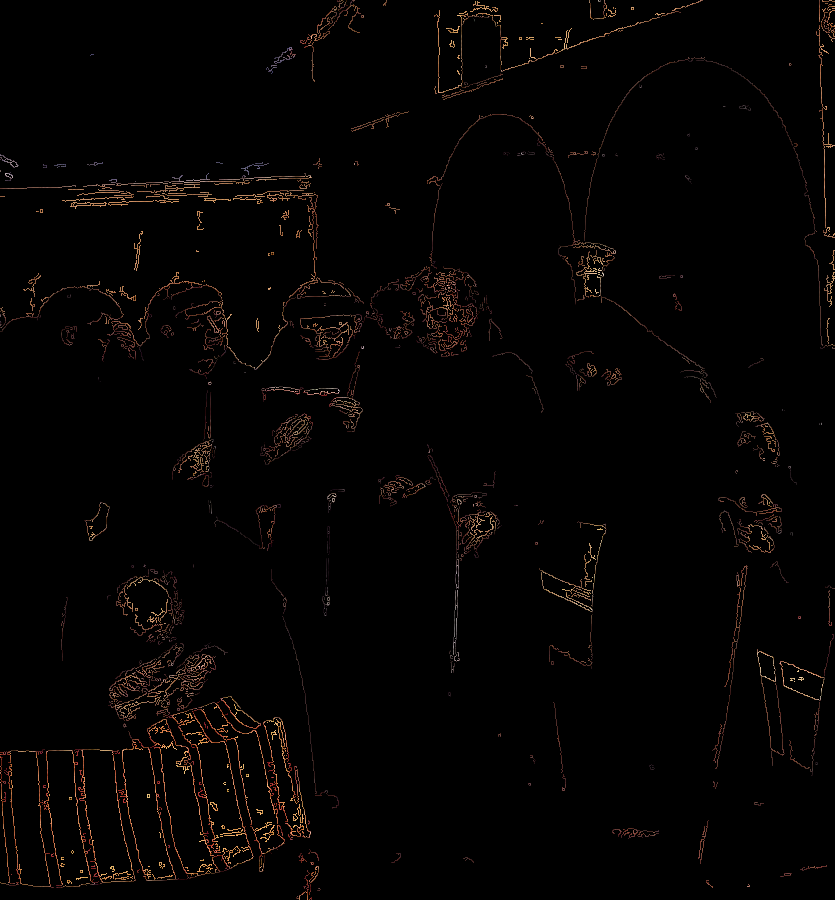
\includegraphics[angle=0,width=0.45\textwidth]{afsnit/afprovning/billeder/thressholds/svage_farver/svage_detalier/2_iteration/100-250.png}
        \label{100-250}}\hspace{1em}
    \subfloat[Orginal]{
        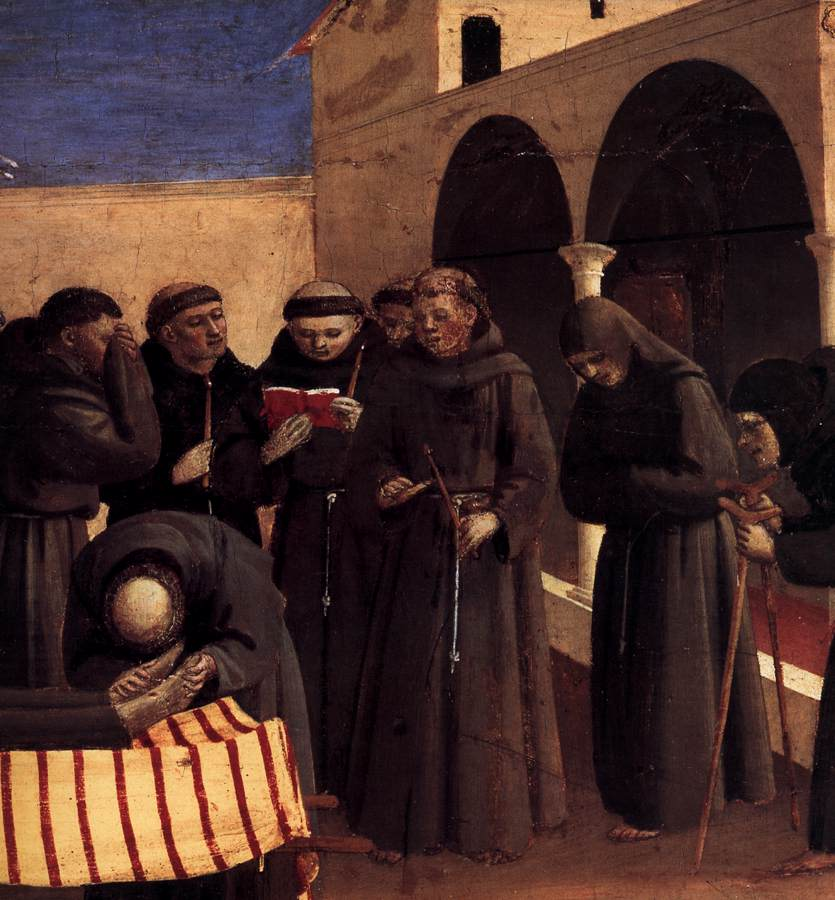
\includegraphics[angle=0,width=0.45\textwidth]{afsnit/afprovning/billeder/thressholds/svage_farver/svage_detalier/sDetalier.jpg}
        \label{Orginal1}}
        \caption[]{Edgedetection på et billedet med svage farver og få detalier, hvor tærskenværdigern [100,250] er den beste}
     \label{en}
\end{figure}

\begin{figure}[!h]
    \centering
    \subfloat[100,240]{
        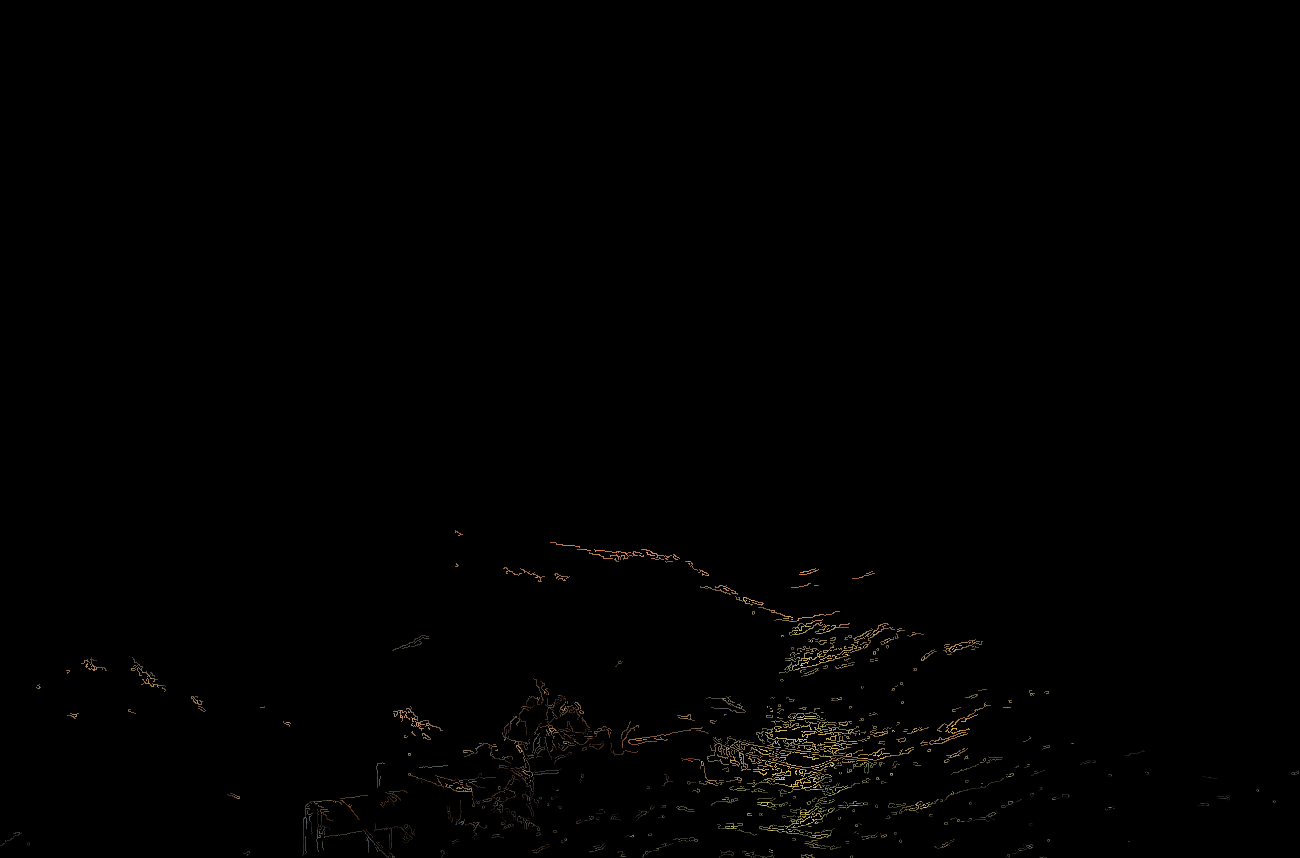
\includegraphics[angle=0,width=0.85\textwidth]{afsnit/afprovning/billeder/thressholds/medium_farver/svage_detalier/2_iteration/100-240.png}
        \label{100-240}}\\
    \subfloat[Orginal]{
        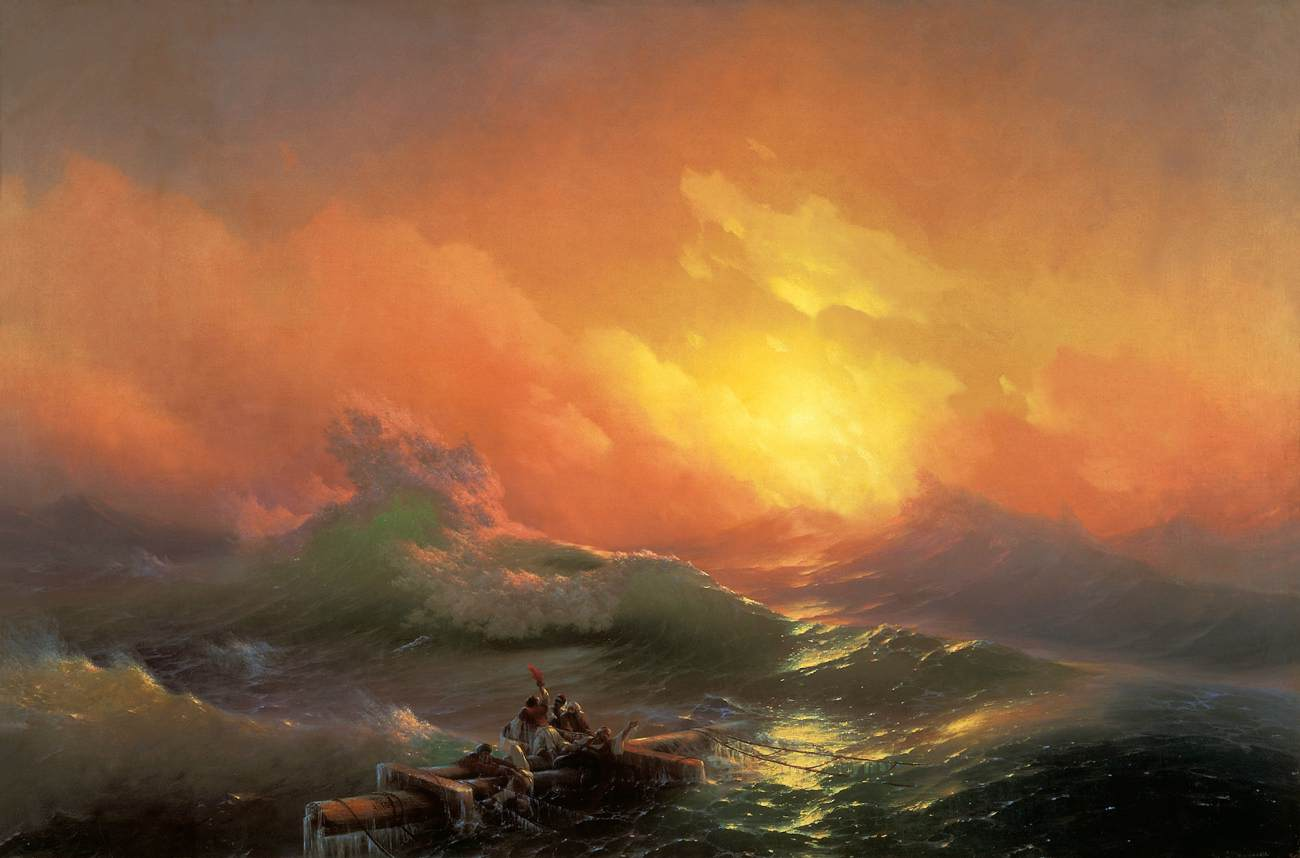
\includegraphics[angle=0,width=0.85\textwidth]{afsnit/afprovning/billeder/thressholds/medium_farver/svage_detalier/sDetalier1.jpg}
        \label{Orginal2}}
        \caption[]{Edgedetection på et billedet med medium farver og få detalier, hvor tærskenværdigern [100,240] er den beste}
     \label{to}
\end{figure}

\begin{figure}[!h]
    \centering
    \subfloat[200,460]{
        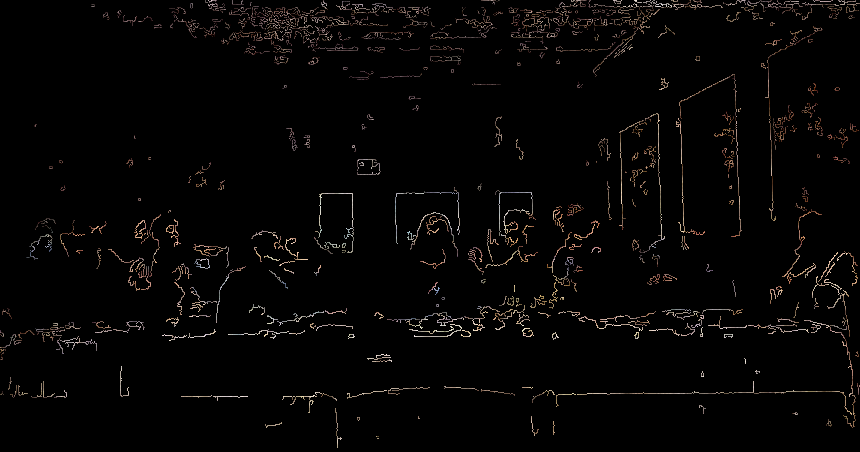
\includegraphics[angle=0,width=0.85\textwidth]{afsnit/afprovning/billeder/thressholds/medium_farver/medium_detalier/2_iteration/200-460.png}
        \label{200-460}}\\
    \subfloat[Orginal]{
        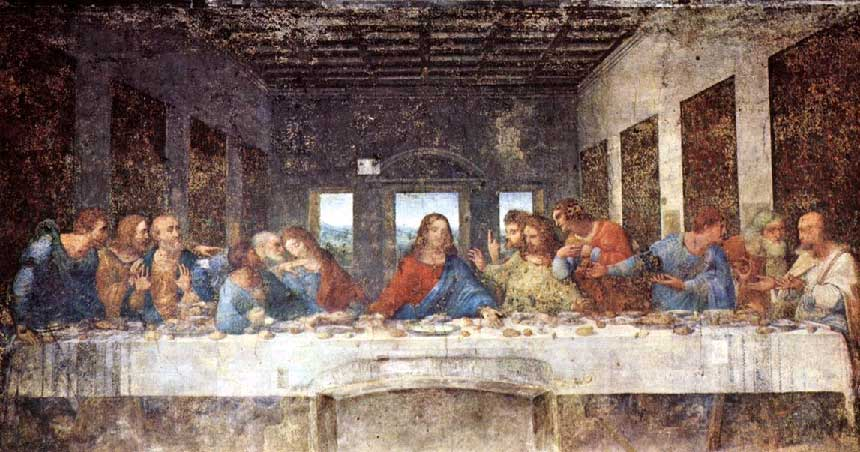
\includegraphics[angle=0,width=0.85\textwidth]{afsnit/afprovning/billeder/thressholds/medium_farver/medium_detalier/mDetalier1.jpg}
        \label{Orginal3}}
        \caption[]{Edgedetection på et billedet med medium farver og medium detalier, hvor tærskenværdigern [200,460] er den beste}
     \label{tre}
\end{figure}

\begin{table}[!h]
    \centering
    \begin{tabular}{| l | l | l | l |} \hline
        & Svage farver 	& Medium farver & Kraftige farver \\ \hline
        Få detalier 		& [100,250]		& [100,240]		& [200,320]\\ \hline
        Medium detalier 	& [100,280]		& [200,460]		& [200,380]\\ \hline
        Mange detalier		& [200,400]		& [200,380]		& [300,750]\\ \hline
    \end{tabular}
    \caption{Beksriv!}
    \label{thressholdsTabelKant}
\end{table}

Som man kan se at tabel \ref{thressholdsTabelKant} gå tærskelværdierne
fra [100,240] til [300,750], så vi kan ikke umiddelbart sætte en fast
tærskelværdi for alle malerier og få at lave en rigtige undersøgelse af
tærskelværdi på malerierne, bliver man nød til at se på mangle flere
malerierne og bestemme deres tærskelværdi og udregne median af de
værdiger, men det vil krave en støre undersøgelse som vi ikke har valt
at gøre, af 3 grunde. 1, det vil kun være en median tærskelværdi få lige
det sæt malerier som vi arbejder på. 2 det vil krave at vi gennemgik
XX(hvor mange) billeder. 3, selv med en median tærskelværdi vil der
stadig være en stor rigge malerier hvor median tærskelværdien ikke vil
være særlige god for. En anden fremgang måde er at regne
tærskelværdierne løbene ud for vært billedet via et program. Men det
problem falder uden for denne opgave og vi vil derfor ikke komme ind på
det. Selv om vi måske ikke kan få det vi helst vil have er der stadig en
del observationer som kan laves ud fra tabellen
\ref{thressholdsTabelKant}. Tærskelværdierne bliver højre nu flere
detaljer og nu kraftigere farverne er. Det virker også som om mange
detaljer vægter lige højt i forholdt til tærskelværdierne en kraftige
farver. Den anden tærskelværdi er ca 2.5 gangen støre en den første
tærskelværdi.

De tærskelværdier som vi har fundet svare til de optimale
tærskelværdier for maleriet, men vi kan godt bruge en værdig som ligger
laver, da metoden floodfill som gør brug af kandtdetektionen resultatset,
god kan tage højde for små kanter, men fejler hvis der ikke er nogle.
Derfor har vi valt at bruger den nederste tærskelværdi som vi har fundet
[100,240] og sænke den lidt til $[78,78 \cdot 2.5 ]$.

\subsection{Afvigelsen af farver i floodfill}
Floodfill har 2 tærskelværdier $lo$ og $up$, som betegner hvor mange pixel
værdier en nabo pixel farver må variere ned og op, en fyldestgørelses
beskrivelse af floodfill findes i afsnit \ref{floodfill}. Vi har tænkt os at
finde en fældes tærskelværdi til brug i vores program. Måde vi gør det på at
ved at observere hvordan floodfill virker med forskellige tærskelværdier og
finde de tærskelværdier som passer bæst til maleriet. Resultatet for
observationen kan ses i tabel \ref{thressholdsTabelFF}, hvor de 9 sammen
kategorier er vist. Et af de malerierne hvor den optimale tærskelværdi er
fundet se i figur \ref{Floodfillbilledet}, så man kan se hvad vi har vurderet
til at være den beste værdi.

\begin{figure}[!h]
    \centering
    \subfloat[8,8]{
        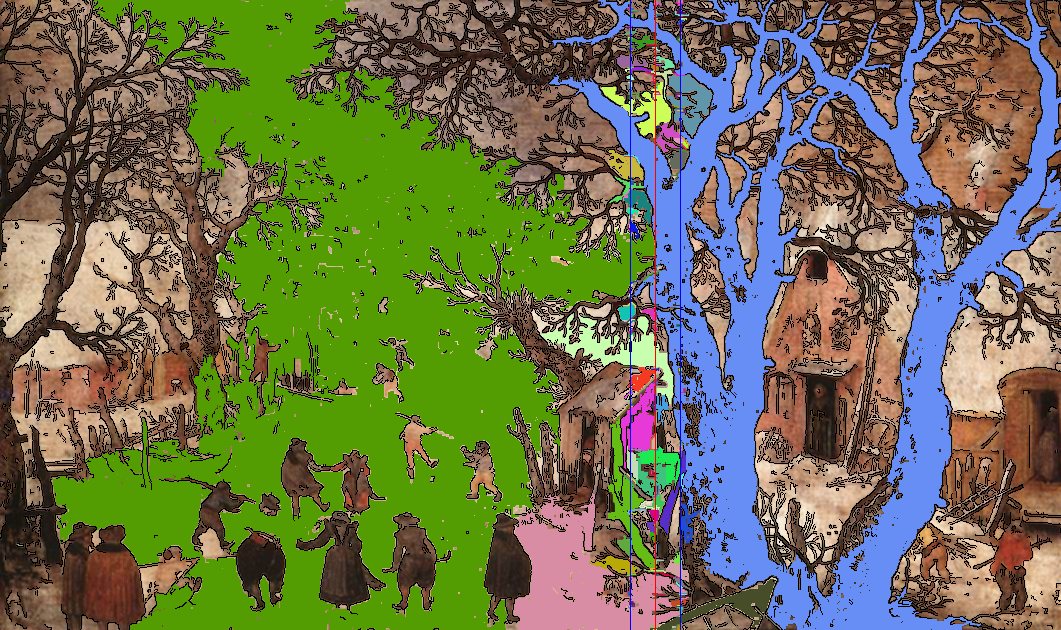
\includegraphics[angle=0,width=0.9\textwidth]{afsnit/afprovning/billeder/thressholds/svage_farver/kraftige_detalier/floodfill/8-8.png}
        \label{8-8}}\\
    \subfloat[Orginal]{
        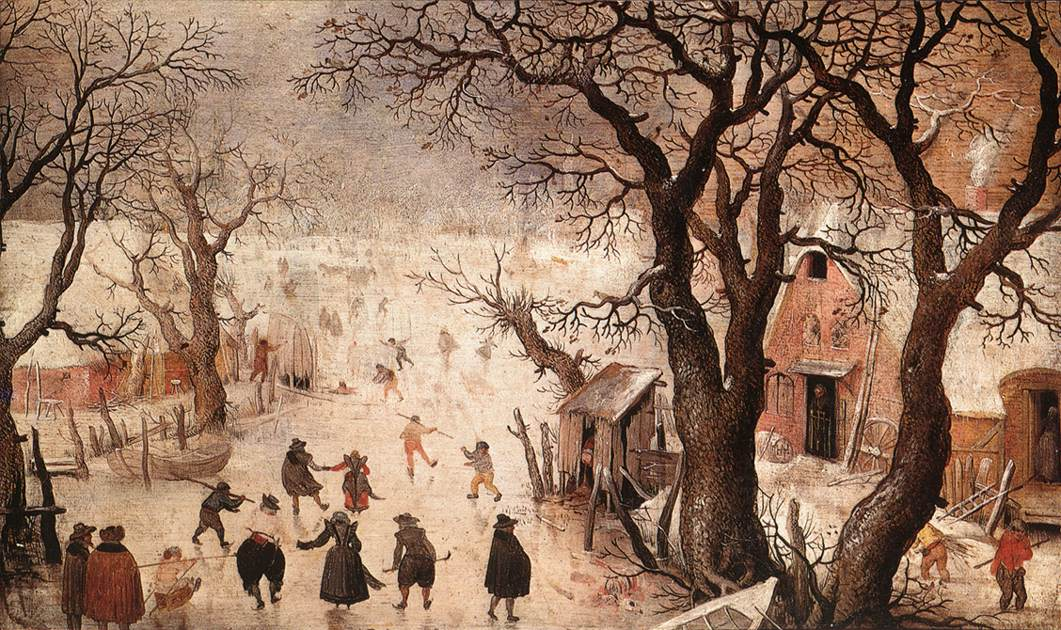
\includegraphics[angle=0,width=0.9\textwidth]{afsnit/afprovning/billeder/thressholds/svage_farver/kraftige_detalier/kDetalier.jpg}
        \label{Orginal4}}
    \caption[]{tærskelværdierne på et billedet med svage farver og kraftige detaljer hvor tærskelværdien [8,8] passer best}
    \label{Floodfillbilledet}
\end{figure}

\begin{table}[!h]
    \centering
    \begin{tabular}{| l | l | l | l |} \hline
        & Svage farver 		& Medium farver & kraftige farver \\ \hline
        Få detalier 		& \textbf{[2,2]}	& [3,3]			& [4,4]\\ \hline
        Medium detalier 	& \textbf{[2,2]}	& \textbf{[5,5]}& \textbf{[2,2]}\\ \hline
        Mange detalier		& [8,8]				& [4,4]			& [7,7]\\ \hline
    \end{tabular}
    \caption{Beskriv!}
    \label{thressholdsTabelFF}
\end{table}

Som man kan af tabellen er nogle af vadierne med fed, begrundelsen for det er
at de vadier er de beste vi kunne finde for billedet, men at de vadier stadig
ikke giver noget som er særlige brugbart, se sektion \ref{floodfilltest}.
værdigerne i tabel fluktuere også en del, så vi har igen samme problem stilling
som i tærskelværdierne ved kantdetektion og har valt at bruge tærskelværdien
[4,4] da dette kommer tættest på gennemsnit.

\clearpage

\subsection{Sløring}
I forbindelse med sløring vil vi gerne teste tre forskellige størrelser på foldningsmatricen der bruges. Vi vil teste
på de sammen ni malerier som i afsnit \ref{terskelverdi}.

\begin{table}[!h]
    \centering
    \begin{tabular}{| l | l | l | l |} \hline
                            & Svage farver	& Medium farver	& Kraftige farver 	\\ \hline
        Få detaljer 		& $(7 \times 7)$	& $(7 \times 7)$	& $(7 \times 7)$		\\ \hline
        Medium detaljer 	& $(5 \times 5)$	& $(7 \times 7)$	& $(7 \times 7)$		\\ \hline
        Mange detaljer		& $(5 \times 5)$	& $(5 \times 5)$	& $(7 \times 7)$		\\ \hline
    \end{tabular}
    \caption{Tabel over hvilke sløringer der er bedst til hvert af sine billeder}
    \label{sloringTabel}
\end{table}

Som man kan se af tabel \ref{sloringTabel} ligger tærskelværdierne på
$(5 \times 5)$ og $(7 \times 7)$, med en svær overvægt af værdierne hen
mod $(7 \times 7)$. I vores program har vi brugt $(3 \times 3)$ da denne
værdi, passer bedst til de billeder vi så på først. Vi har valgt ikke at
vise nogle eksempler, da sløringerne ikke ses særlige godt i nedskaleret
billeder, og at et eksempel er givet i figur \ref{simple_metode}

\clearpage

\subsection{Rigtige undersøgelse}
I de afprøvninger vi har gjort, har vi brugt ni malerier, til at være
repræsentativ for resten af malerierne i kunstdatabase. Vi har også selv
valt de ni malerier, ud for kriteriet at der skulle være alsidighed og at
man skal kunne vise problem stilinger visuelt ud af afprøvning på
malerierne.

Denne metode virker også godt, nå vi gerne vil ud med nogle pointer.
Men for at lave en mere statistiske signifikant undersøgelse for det
datasæt. Burte vi teste en del flere billeder, lad os sige 50 og
så bagefter teste på 100, og så se om der dannet sig et mønster. 

Vi burte også delle billederne op i grupperinger, f.eks. maleriets
oprindelse og så udvælge test malerierne efter ca samme procents vise
fordeling, så hvis kunstdatabasen består af $15 \%$ malerier fra
Italien, så skal der også være ca $15 \%$ Italienske malerier i test
malerierne.

Til sidest burte malerierne også vælges tilfældig ud inde for deres
grupperinger

Grunden til at vi ikke har gjort det på denne måde er, af tre grunde

\begin{enumerate}
	\item Det vil stadig kun være en undersøgelse for lige det sæt
	malerier som vi arbejder på og ikke andre data materiale.
	\item Det vil krave afprøvning på mange malerier, som vi ikke har
	resurser til. 
	\item Selv med en gennemsnit tærskelværdi fra et statistisk
	signifikant undersøgelse vil der stadig være en stor rigge malerier
	hvor gennemsnit tærskelværdien ikke vil være særlige god for. 
\end{enumerate}


\subsection{Overvejlser om tærskelværdier}
En anden fremgangsmåde til problemstillingen med tærskelværdier, kunne
være at regne tærskelværdierne løbende ud for billede. Det ville
løsen en masse af de problemer som vi støder på. Men det problem falder
uden for denne opgave.



\section{Regions detektor\label{region_detektor}}
I dette afsnit vil vi afprøve den generelde region detektor, det vil
sige hvad der egentlig bliver fundet inden, vores to metoder sortere
regionerne fra. selve metodes fremgangsmåde er beskravet i sektion
\ref{Sammensetning_af_metoder}, hvor det sideste skrid nå billedet
bliver floodfilldet, derfor vil vi forklare afprøvningen af metode ud
fra billeder som er kommer til dette skridt, hvor tærskelværdierne er
sat til de fundene tærskelværdier. Den første del vil omhandle test på
opbygget billeder og den anden del vil omhandle test på udvalgte
billeder fra vores billedet database.

\subsection{Afprøvning på test billeder}
I dette sektion tester vi på billeder som er konstrueret, men en hvid
baggrund og sorte regioner, det snit vi tester på er indtegnet samt
marginen. I billedet \ref{GRD_test1} er der 5 regioner, hvor 3 af dem bliver
fundet da de ligger i snittet, de 2 regioner som ikke er fundet er
stadig sorte, som man kan se bliver både den er krydser snittet og den
der tangere snittet taget med. I billedet \ref{GRD_test2} er der 3 regioner som
alle bliver fundet, baggrunden, den lille region som ligger inde for
margin, og den store region som kun har en lille del af dens masse inde
i snittet. I billedet \ref{GRD_test3} er der en hoisont som ligger oven på
snittet, begge sider af hoisont linien bliver tegnet med.


\begin{figure}[!h]
    \centering
		\subfloat[4 figure og en bagrun, hvor 2 af figurene og bagrunden er fundet]{
        	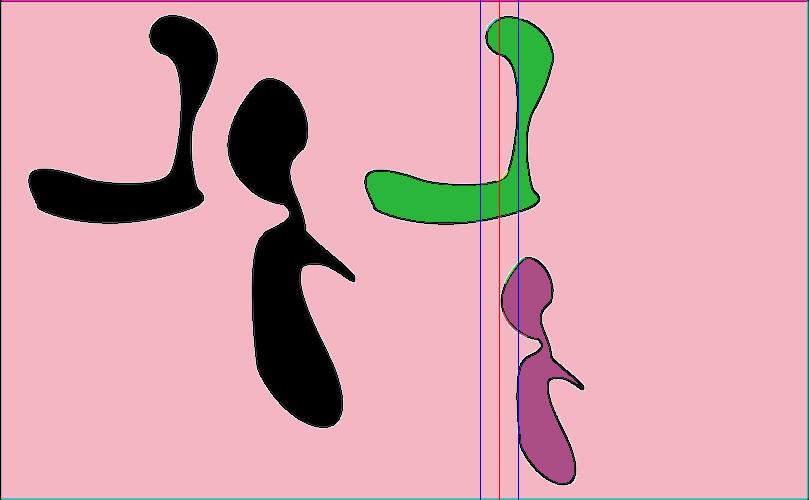
\includegraphics[angle=0,width=0.7\textwidth]{afsnit/afprovning/billeder/region_selector/blob_region_section.png}
        	\label{GRD_test1}}\hspace{1em}
    		\subfloat[En stor figur og en lille figur begge fundet]{
	        	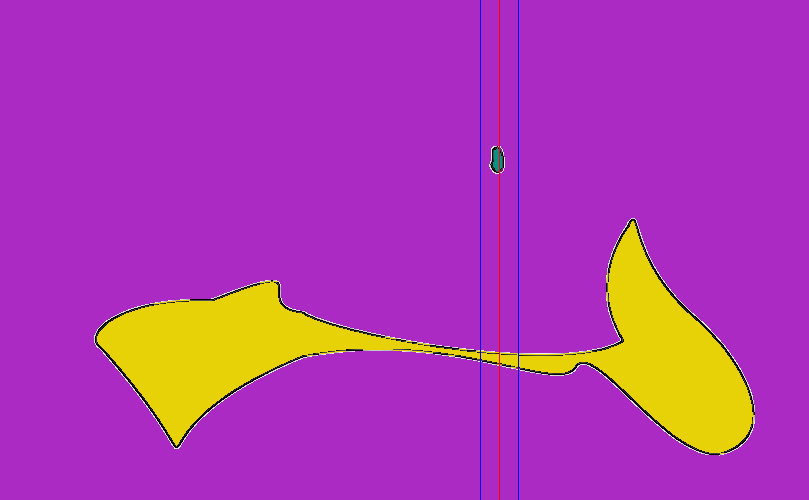
\includegraphics[angle=0,width=0.7\textwidth]{afsnit/afprovning/billeder/region_selector/blob2_region_section.png}
	       	\label{GRD_test2}}\hspace{1em}
    		\subfloat[En hoisont, hvor begge sider er fundet]{
	        	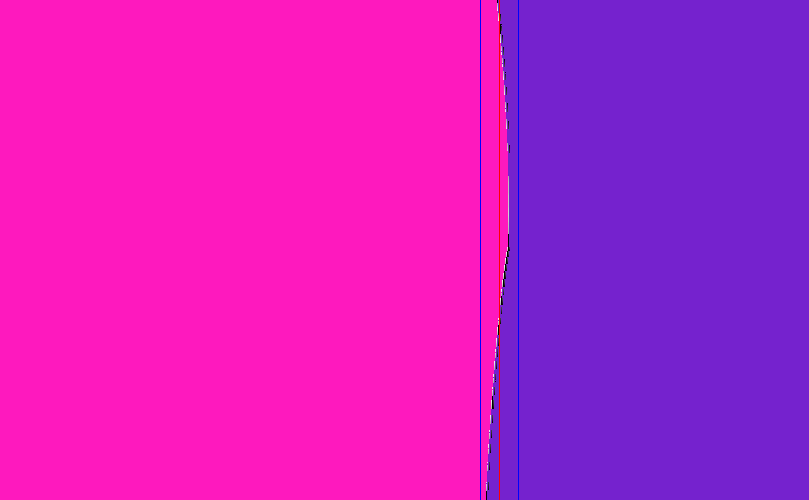
\includegraphics[angle=90,width=0.5\textwidth]{afsnit/afprovning/billeder/region_selector/hoisont_region_section.png}
		       	\label{GRD_test3}}\hspace{1em}
        \caption[]{3 test billeder med bløde former, hvor regien detektor er kørt på dem}
     \label{region_detektor_test}
\end{figure}

I figur \ref{region_detektor_test} er de 3 test billeder afbilledet, de
opføre sig efter de standarter som vi frem satte i afsnit
\ref{}XX(hvilken reference?) 

\subsection{Afprøvning på malerier}
Vi vil afprøve region detektor på 6 udvalte billeder, som vær viser
styrker og svagheder ved region detektoren

\begin{figure}[!h]
    \centering
		\subfloat[Maleri med Kraftige farver og få detaljer]{
        	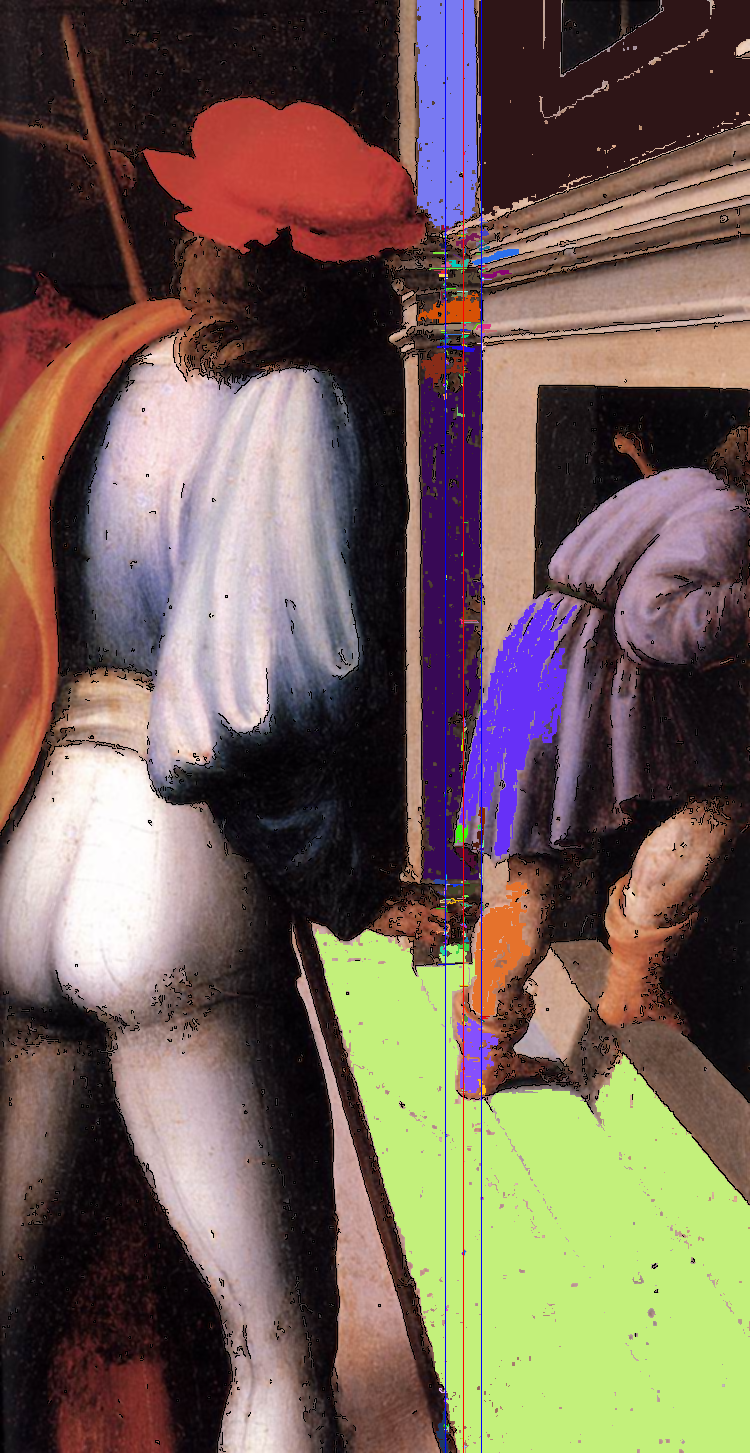
\includegraphics[angle=270,width=1.0\textwidth]{afsnit/afprovning/billeder/thressholds/krafitige_farver/svage_detalier/floodfill/4-4.png}
        	\label{GRD_virker1}}\hspace{1em}
		\subfloat[Medium farver og medium detaljer]{
        	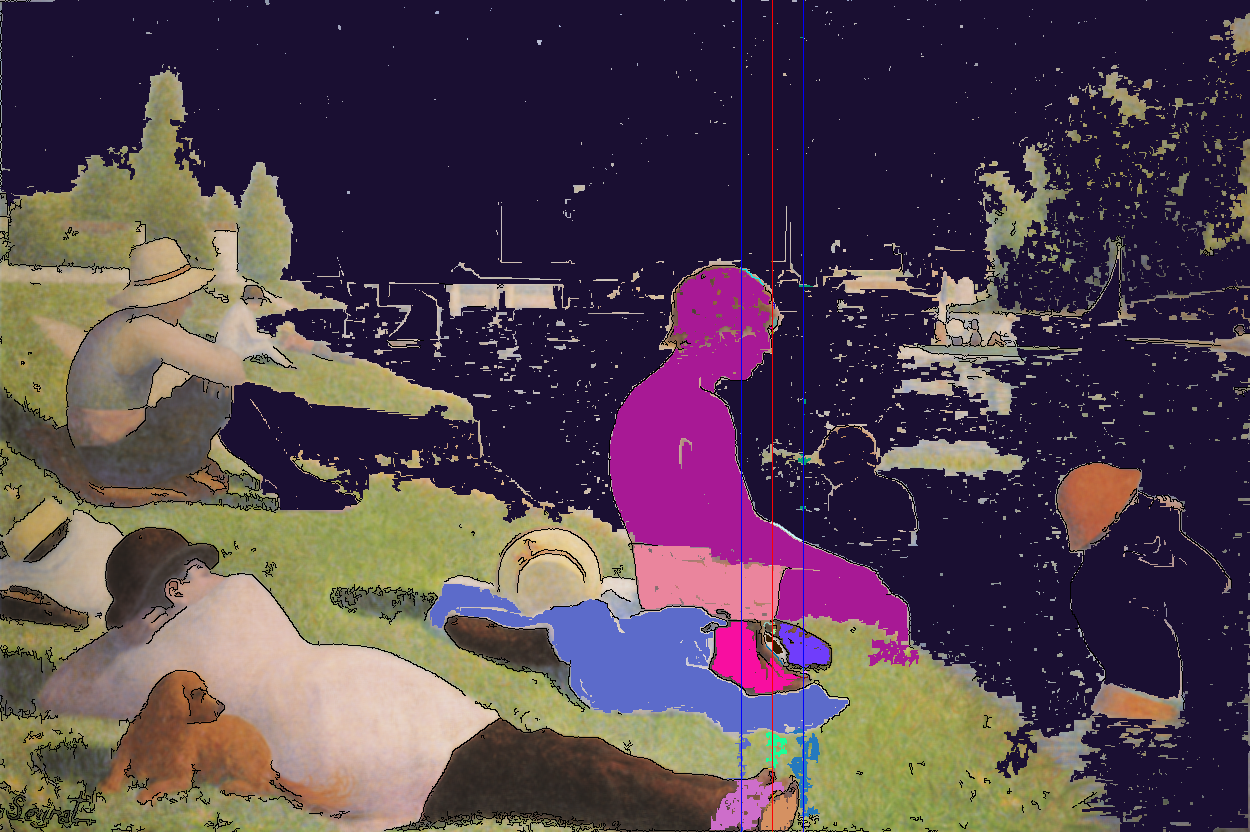
\includegraphics[angle=0,width=1.0\textwidth]{afsnit/afprovning/billeder/4-4.png}
        	\label{GRD_virker2}}\hspace{1em}
        \caption[]{2 malerier hvor regions detektoren virker efter vores ønsker}
     \label{generelde_region_detektor_virker}
\end{figure}

I figuren \ref{generelde_region_detektor_virker} er der 2 malerier, hvor
vores region detektor virker rigtige godt, det første maleri
\ref{GRD_virker1} finder region detektoren 7 store regioner og en masse
små, metoden finder forskel på de forskellige paneler i kaminen og vært
tøj stykke på personen i maleriet er blevet vær deres region, de små
regioner er samlet ved et skift fra et panel til et andet og forstyrrer
ikke de store region ved at gå i gennem dem, man kunne måske have ønsket
at den fylde lidt mere af han karpe ud, men eller et meget godt eksempel
på hvordan den generelde region detektor finde lige det vi vil have den
til at finde. I maleriet \ref{GRD_virker2} finder vi mange af de samme
godt ting, drengen i miden af maleriet er helt udfyldt, en sko og et
håndklæde er også fundet, det er dog vigtigt at ligge mærke til at de
andre personer i vandet, fylder i et med baggrunden, som normalt vil
være en dårlig ting, men som ikke gør noget her da, metoden kun ser
efter regioner i snittet, repræsenteret af den røde linie.
 
\begin{figure}[!h]
    \centering
		\subfloat[Kraftige farver og mange detaljer]{
       	 	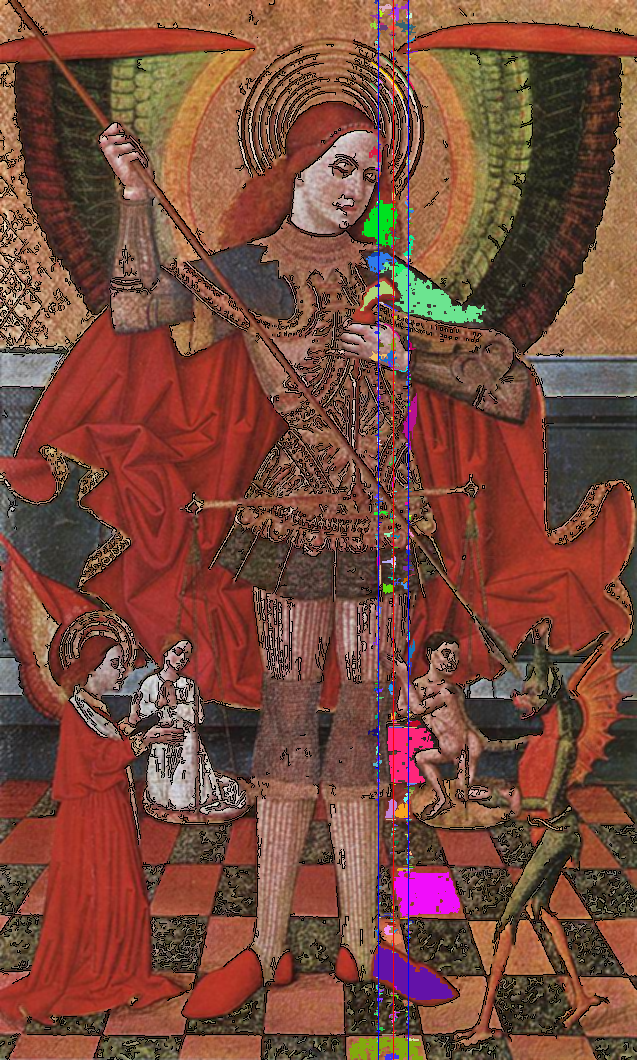
\includegraphics[angle=270,width=0.90\textwidth]{afsnit/afprovning/billeder/thressholds/krafitige_farver/krafite_detalier/floodfill/4-4.png}
		    \label{GRD_virker_nesten1}}\hspace{1em}
    \subfloat[Medium farver og medium detaljer]{
        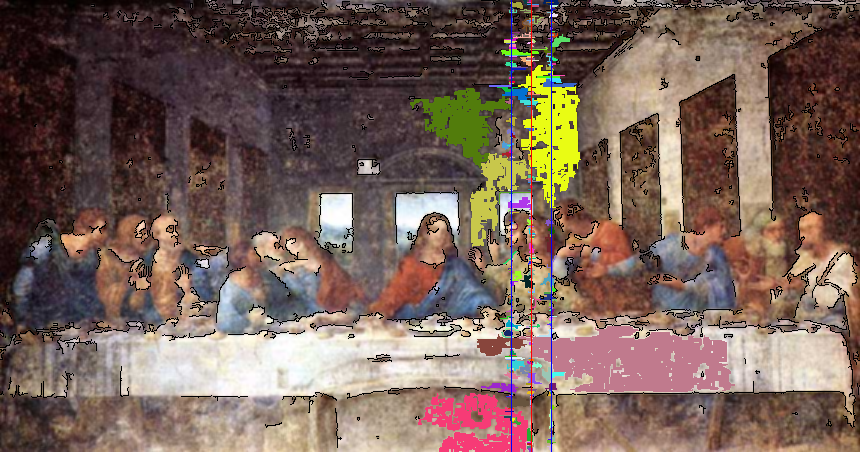
\includegraphics[angle=0,width=0.95\textwidth]{afsnit/afprovning/billeder/thressholds/medium_farver/medium_detalier/floodfill/4-4.png}
        \label{GRD_virker_næsten2}}\\
     \label{generelde_region_detektor_virker_nesten}
     \caption[]{2 malerier hvor regions detektoren ikke helt virker efter vores ønsker men stadig har noget vi kan bruge}
\end{figure}

I figuren \ref{generelde_region_detektor_virker_nesten} er der 2
malerier, hvor vores region detektor ikke virker efter vores ønsker med
stadig har noget vi kan bruge, I maleriet \ref{GRD_virker_nesten1}
bliver der mest fundet små region dog bliver en sko, en skulder og en
flise fundet, hvor vi gerne vil have at personens karpe og arm også blev
fundet, dette skyldes primert at tærskelværdierne for dette billedet er
sat for lavt. Det andet maleri \ref{GRD_virker_nesten2} har nogle af de
samme problematiker, region detektoren finder mest en masse små stykker
af noget som burde hænge sammen. Det vil også kunne løses ved nogle
andre tærskelværdier, men som man også kan se på maleriet er væge og
loftet som egentlige er ret ensfarvet stadig svære for vores region
detektor at fange, det tyder på at en støre sløring godt kunne være
problemløseren få at algoritmen virker på dette maleri. Grunden til at
lige de her 2 bilder er interessante er at ved ændring på tærskelværdier
og sløring kunne vores region detektor virker godt XX(her skal der
billeder hvor det virker), 

\begin{figure}[!h]
    \centering
    \subfloat[Kraftige farver og medium detaljer]{
        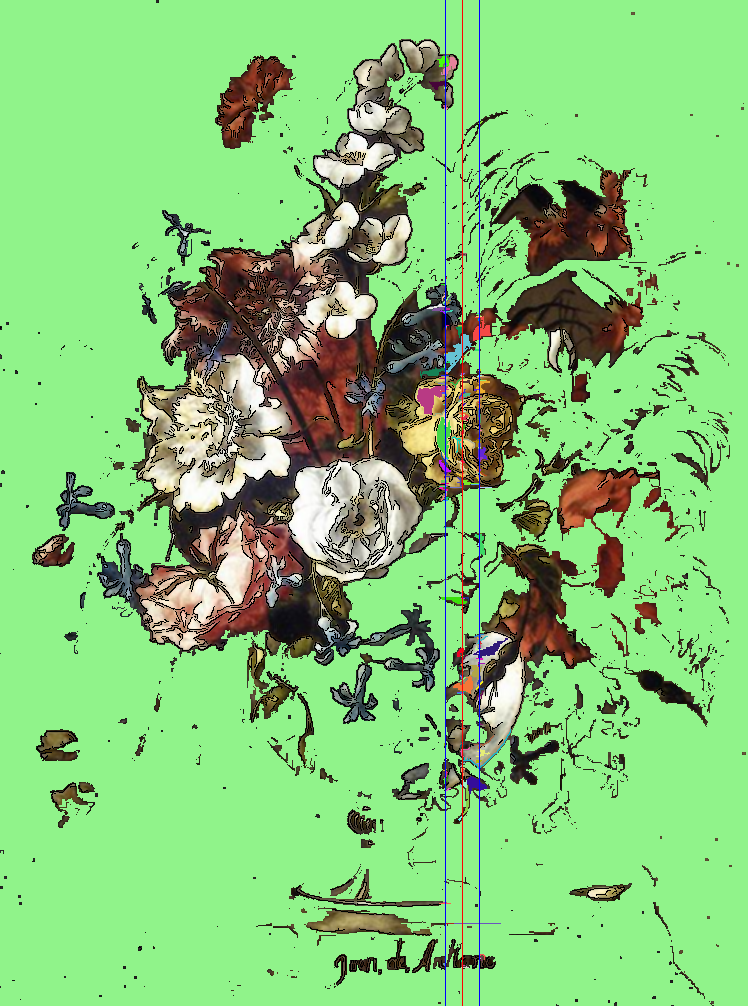
\includegraphics[angle=0,width=0.65\textwidth]{afsnit/afprovning/billeder/thressholds/krafitige_farver/medium_detalier/floodfill/4-4.png}
        \label{GRD_virker_ikke1}}\\
    \subfloat[Svage farver og få detaljer]{
        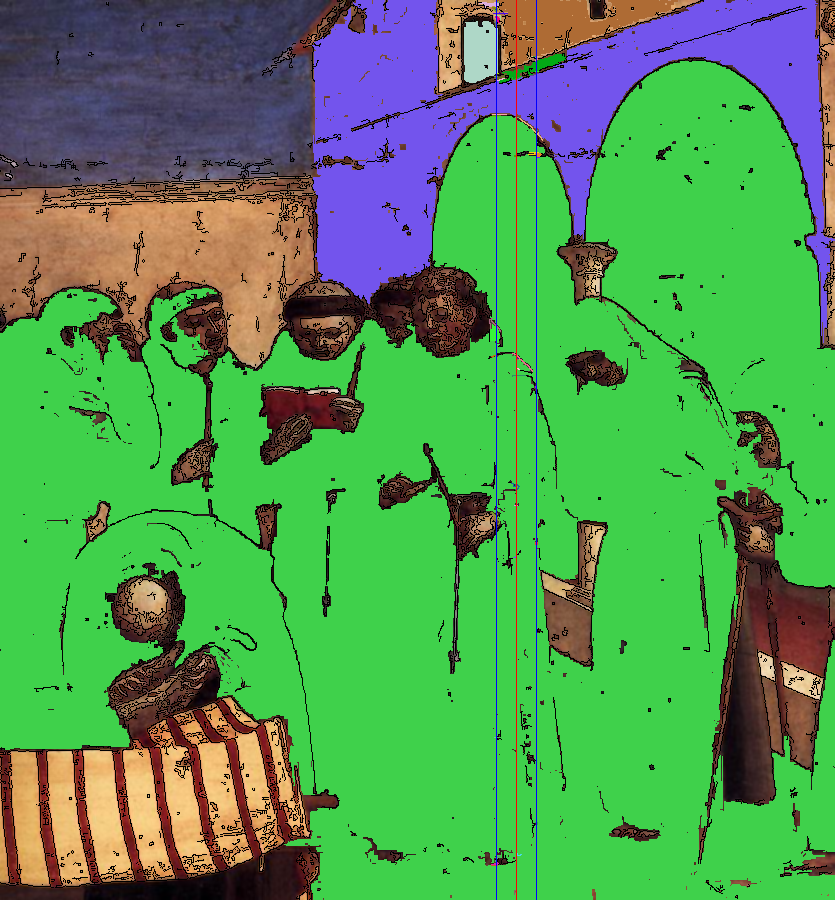
\includegraphics[angle=0,width=0.65\textwidth]{afsnit/afprovning/billeder/thressholds/svage_farver/svage_detalier/floodfill/4-4.png}
        \label{GRD_virker_ikke2}}\hspace{1em}
     \label{generelde_region_detektor_virker_ikke}
\end{figure}

I figur \ref{generelde_region_detektor_virker_ikke} er der 2 malerier
hvor vores region detektor ikke virker særlige godt. I maleri
\ref{GRD_virker_ikke1} er noget af buketten og baggrunden gået i et. På
samme tid er resten af blomsterne i snittet ikke fyldt ud, og selv med
en ændring i tærskelværdierne vil det ikke hjælpe, da en øgning af
tærskelværdierne vil resultere i at flere af blomsterne gå i et med
baggrunden, og en sænkning, vil resultere i at ingen af blomsterne vil
blive detektet. Maleriet \ref{GRD_virker_ikke2} har en anden
problemstiling som vi ikke kan komme uden om, farverne er så mørke og
svage at en ændring i tærskelværdien i floodfill på bare 1 vil få
regiondetektoren til at gå fra at finde ingen regioner til at finde en
stor, som på billedet, dette kan også skyldes at kantdetektionen
tilføje en mørk kan rundt om regionerne, men da maleriet er mørkt i
forvejen hjælper kandetektionen ikke.
XX(jeg kan ikke helt prolamere dette unden at have nogle bileder at bagge det op)


\clearpage


\section{Sortering i interessante regioner}
{\sffamily 
Nå regions detekter, har fundet alle regioner, vil vi gerne sortere ud i
regionerne, da små regioner og regioner med en for lille masse ikke er
interessante for vores 2 metoder.
}


\subsection{Regionstørrelse \label{region_stoerlse}}
%% Bemærk:
%%          Resten af rapporten følger en stil hvor indledninger skrives
%%          med \sffamlily-typen. Denne stil bør ikke bruges her, da dette ikke er \section
%%
I vores region detektor sætter vi en værdi for hvor stor en region skal
være få at blive tage i betrakting, i dette sektion vil vi test,
hvor stor en regionen skal være for at vi vil tage den med. Problemetiken
med få små regioner er illustret i maleri \ref{alt_med} hvor alle de
gråne kasser er en region som vores naive algoritme mener er
interessante, og da alle regioner tage med, bliver 939 regioner godtaget
til at ligge i snittet.

\begin{figure}[¡h]
    \setlength\fboxsep{0pt}
    \setlength\fboxrule{0.5pt}
    \begin{center}
        \fbox{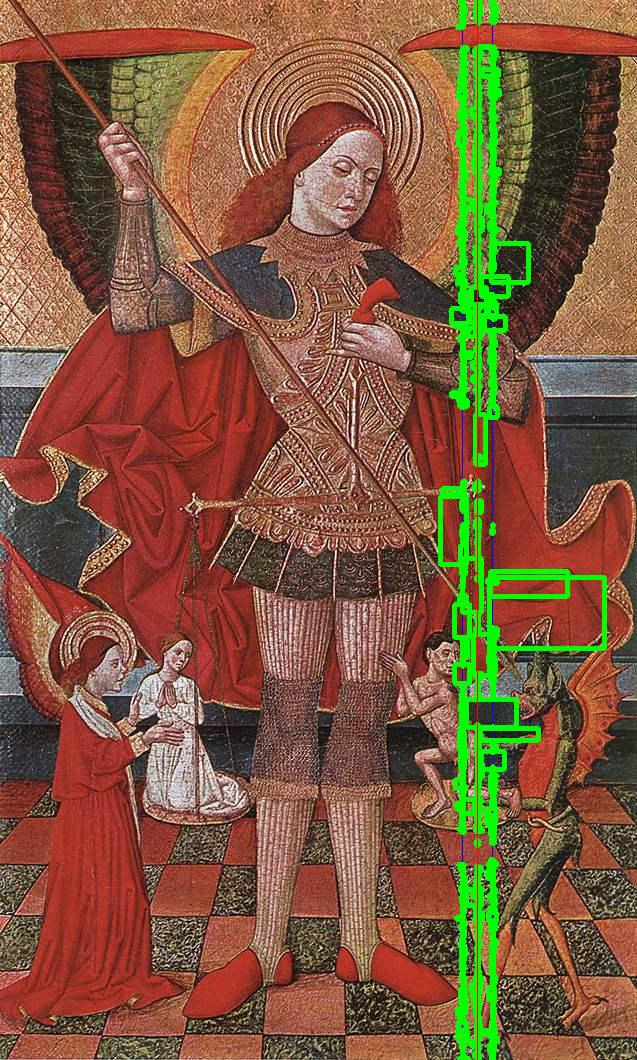
\includegraphics[angle=0,width=0.45\textwidth]{afsnit/afprovning/billeder/stoerelse/alt_med.png}}
    \end{center}
    \caption{Maleri hvor alle størrelse regioner er godtaget, der er fundet 939 intrasante regioner}
	\label{alt_med}
\end{figure}

For at teste hvilken størrelse vi gerne vil godtage er der fremstilet et
testbilledet \ref{original_stoerelse} hvor ni regioner er opstillet så de
alle ligger i sammen snit. Dem øvereste regioner er den minste, og så
stiger regioners størrelse gradvis ned af i billedet.

I vær at de andre fem testbilleder i figur \ref{stoerelse_sammenlining}
er tærskelværdierne gradvis sat op, i testbillederne skal man ligge
mærke til hvilke størrelse regioner der bliver godtaget, representeret
af den grånde kasse. Vi mener at der bliver taget for mange regioner med
i billedet \ref{0,0}, \ref{0,005}, \ref{0,001} og \ref{0,0015}. I
billedet \ref{0,002} vurdere vi at store nok regioner kun taget med, og
vi har derfor valt at sætte tærskelværdien til $0.002$
 
\begin{figure}[!h]
    \setlength\fboxsep{0pt}
    \setlength\fboxrule{0.5pt}
    \centering
    \subfloat[Det original billedet]{
        \fbox{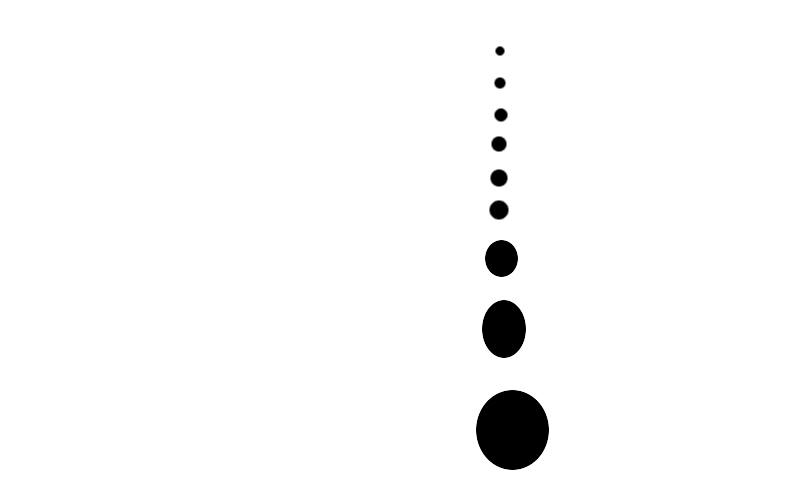
\includegraphics[angle=0,width=0.45\textwidth]{afsnit/afprovning/billeder/stoerelse/stoerelse.png}}
       \label{original_stoerelse}}
    \subfloat[Tærskelværdien sat til 0]{
        \fbox{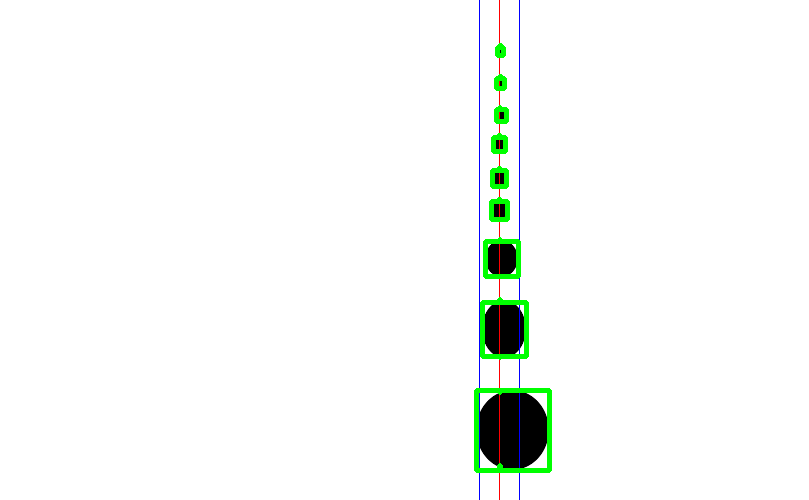
\includegraphics[angle=0,width=0.45\textwidth]{afsnit/afprovning/billeder/stoerelse/0.png}}
       \label{0,0}}\\
    \subfloat[Tærskelværdien sat til 0.0005]{
        \fbox{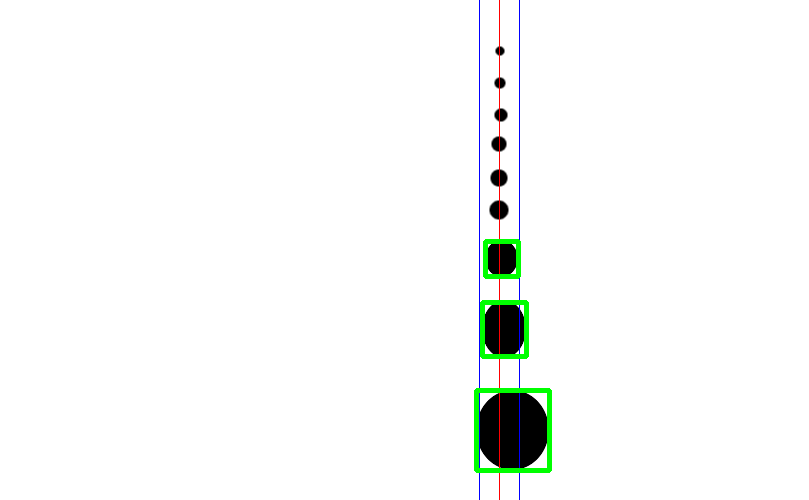
\includegraphics[angle=0,width=0.45\textwidth]{afsnit/afprovning/billeder/stoerelse/0,0005.png}}
       \label{0,005}}
    \subfloat[Tærskelværdien sat til 0.001]{
        \fbox{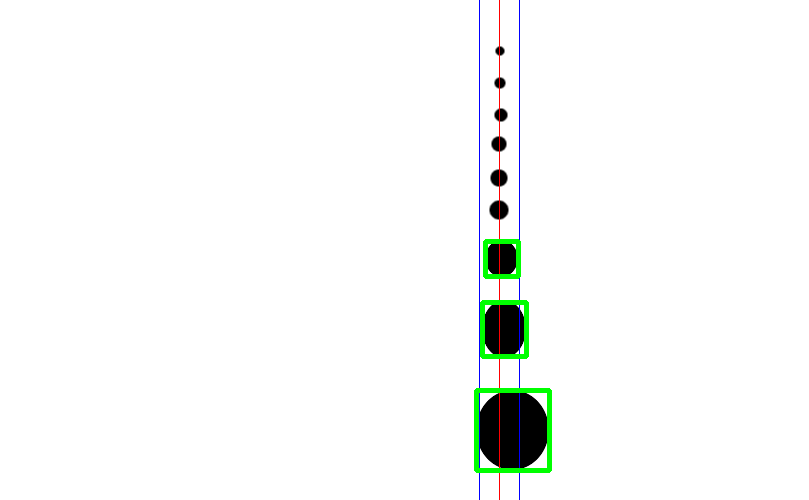
\includegraphics[angle=0,width=0.45\textwidth]{afsnit/afprovning/billeder/stoerelse/0,001.png}}
       \label{0,001}}\\
    \subfloat[Tærskelværdien sat til 0.0015]{
        \fbox{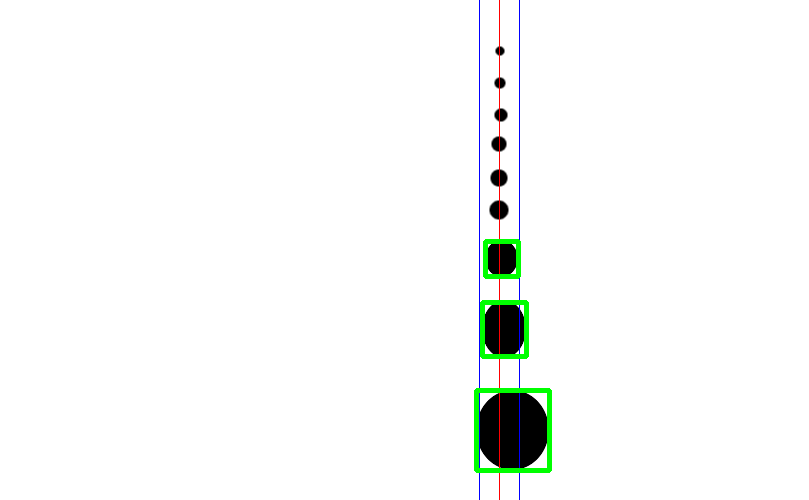
\includegraphics[angle=0,width=0.45\textwidth]{afsnit/afprovning/billeder/stoerelse/0,0015.png}}
       \label{0,0015}}
    \subfloat[Tærskelværdien sat til 0.002]{
        \fbox{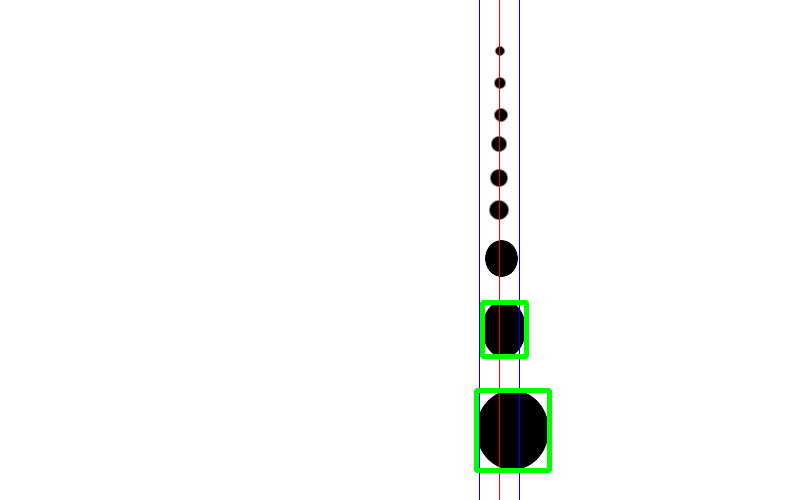
\includegraphics[angle=0,width=0.45\textwidth]{afsnit/afprovning/billeder/stoerelse/0,002.png}}
       \label{0,002}}
    \caption{Testbilledet med ni regioner, som bliver støre og støre. Hvor den originale billedet samt 5 forskellige tærskelværdier er afbilledet}
    \label{stoerelse_sammenlining}
\end{figure}

\clearpage

\subsection{Masse}
For at en region bliver taget i betragtning skal den have en masse som
er støre en vis tærskelværdi, som forklare i \ref{naiv_regler}. På samme
fremgangsmåde som i afsnit \ref{region_stoerlse} sammenligner vi 5
forskellige tærskelværdier og kommer frem til at hvis figurens masse er
under en $\frac{1}{4}$ af afgrænsende rektangel, vil vi ikke tage den
med. En illustrere af hvad vi vælger at tage med kan ses i figur
\ref{mass}, hvor region detektoren er kørt på billedet
\ref{naiv_masse_original} og resultatet kan ses i figur \ref{naiv_masse}

\begin{figure}[!h]
    \centering
		\subfloat[2 regioner hvor den ende er sorteret vær på grund af dens masse]{
	        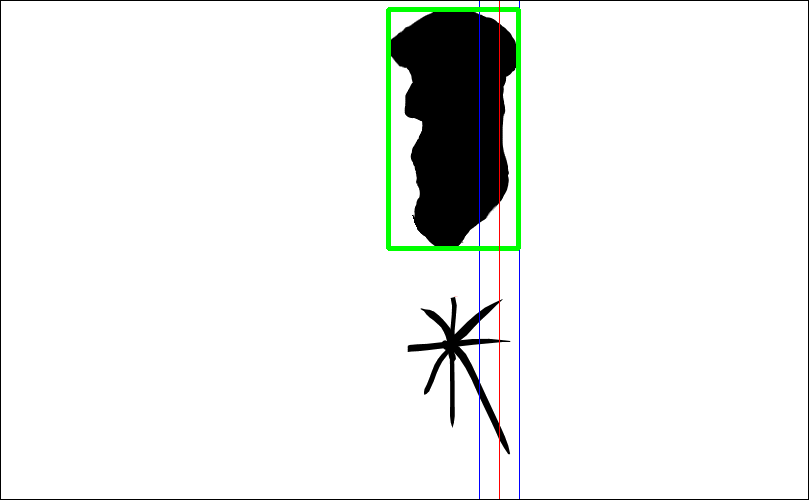
\includegraphics[angle=0,width=0.55\textwidth]{afsnit/afprovning/billeder/naive_losning/naiv_mass.png}
	       	\label{naiv_masse}}\hspace{1em}
	    \subfloat[Original]{
	        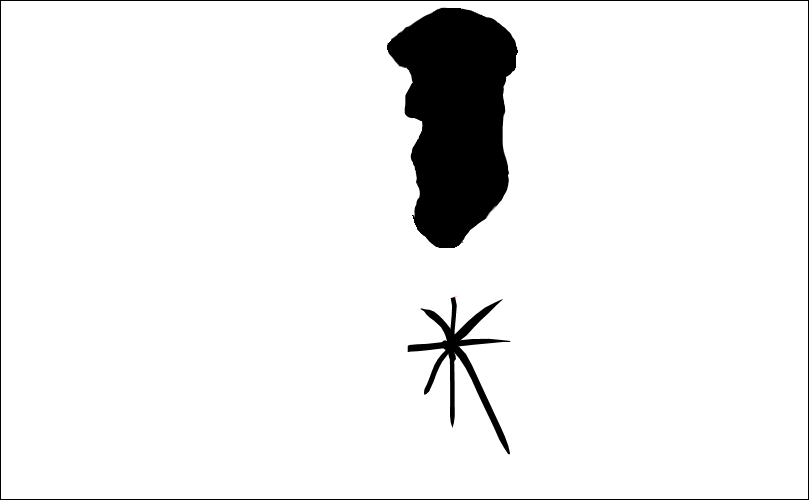
\includegraphics[angle=0,width=0.55\textwidth]{afsnit/afprovning/billeder/naive_losning/mass.png}
	       	\label{naiv_masse_original}}\hspace{1em}
		\label{masse}
\end{figure}

\clearpage

\subsection{Overvejlser om regions detektoren}
Udvælgelsen af interessante regioner, kunne godt, være mere
sofistikeret.  Vi undersøger kun regioner for deres størrelse og masse,
hvilket stadig tillader mange regioner, som egentlig er uinteressante,
pga. deres form.  I udvælgelsen af interessante regioner, kunne man
derfor kigge på regionens form eller udstrækning, ved at undersøge
dennes massemidtpunkt.  Hvis massen er koncentreret langt væk fra
snittet, er denne region ikke interessant. Vi skal dog passe på, at vi
ikke tager beslutninger, som egentlig vedrører, om regionen er placeret
i snittet. Vi ønsker, i denne udvælgelse af regioner, udelukkende at
bestemme, hvorvidt regionen skal tages op til videre overvejelse, for om
denne ligger i snittet.

Kun hvis vores søgning for objekter i billedet, bliver mere specifik,
giver det mening, at undersøge regionerne nærmere i udvælgelsen af
interessante regioner. Vi kan forestille os, en situation, hvor man
udelukkende vil finde ansigter, placeret i det gyldne snit. I dette
tilfælde, skal vi selvfølgelig ikke sende en region til videre
vurdering, hvis denne \emph{ikke} er et ansigt. Vi har dog ikke en sådan
specifik søgning, hvorfor vi kun kan frasortere regioner, ud fra
informationen om deres størrelse og masse.




\section{Naive løsning}
%% Bemærk:
%%          Resten af rapporten følger en stil hvor indledninger skrives
%%          med \sffamlily-typen. Denne stil bør også følges her.
%%
{\sffamily
I dette sektion vil vi teste den naive løsning. ved at se om den sortere
de rigtige regioner væk og om løsningen opføre sig på samme måde som vi
har håbet på. Det vil vi gøre ved ført at se på nogle fabrikeret test
billeder, får at se om den naive løsning virker efter meningen og
bagefter vil vi teste på malerierne for at se om den naive løsning kan
bruges i praktisk.
}
  
\subsection{Afprøvning på testbilleder}
Vi vil teste på de samme testbilleder som i sideste afsnit, samt et nyt
testbilleder som blev brugt i forklaringen af den naive metodes, de fire
billeder som vi har valt at test kan se i afsnit \ref{region_detektor}
og billedet \ref{naiv_masse_original} hvor en grån kasse rundt om en
region, betyder at den er valt til at ligge i det gyldne snit af den
naive metode. 

Det første billedet \ref{naiv_blob1}, har fem regioner og hvor tre af
dem blev fundet af reginon detektoren, vores naive løsning har så
sorteret baggrundens regionen og den øverste region i snitte vær, da de
begge krydser marginer og derfor ikke overholder definition
\ref{} . 

\begin{figure}[!h]
	\begin{center}
        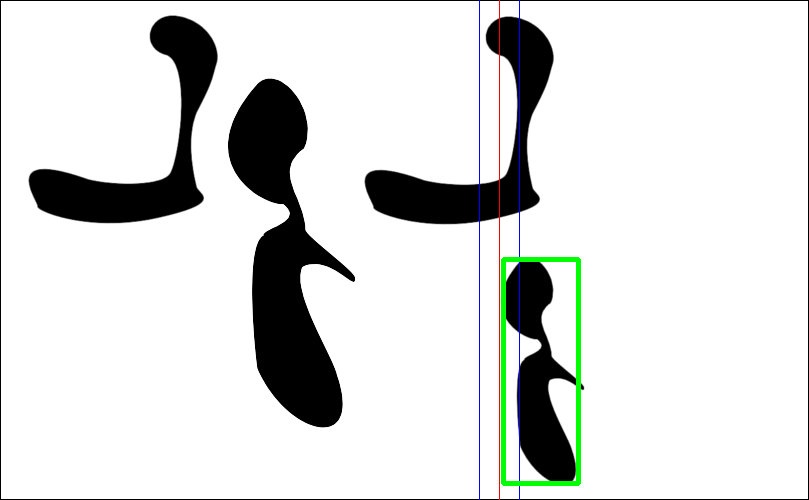
\includegraphics[angle=0,width=0.55\textwidth]{afsnit/afprovning/billeder/naive_losning/naiv_blob1.png}
	\end{center}       
	\caption{Naive algoritme finder en ud af fem regioner}	
	\label{naiv_blob1}
\end{figure}

Det andet billedet \ref{naiv_blob2}, er alle blevet sorteret vær, også
den lille, da den er for lille, derfor ikke overholder definition
\ref{def_interessant} b. 

\begin{figure}[!h]
	\begin{center}
       	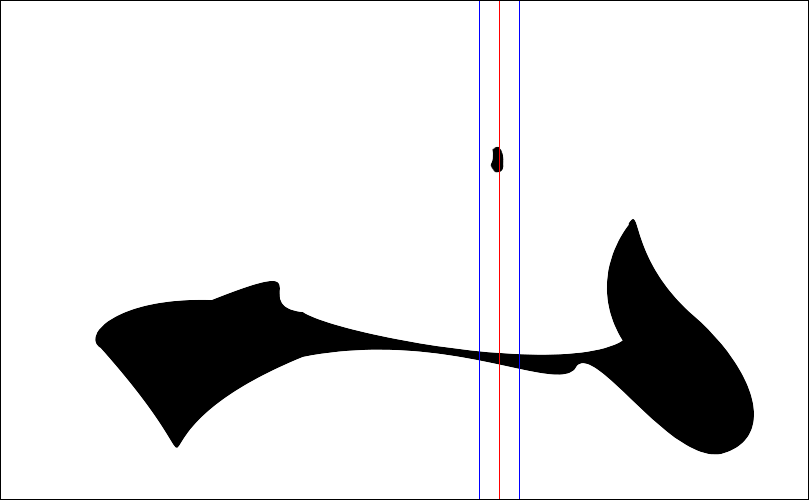
\includegraphics[angle=0,width=0.55\textwidth]{afsnit/afprovning/billeder/naive_losning/naiv_blob2.png}
	\end{center}
	\caption{Værgen den lille region eller den store er fundet} 
   	\label{naiv_blob2}
\end{figure}

I test billedet \ref{naive_hoisont1}, sortere algoritmen
himlen fra, da den krydser margin lidt, men tager jorden med. 

\begin{figure}[!h]
	\begin{center}
       	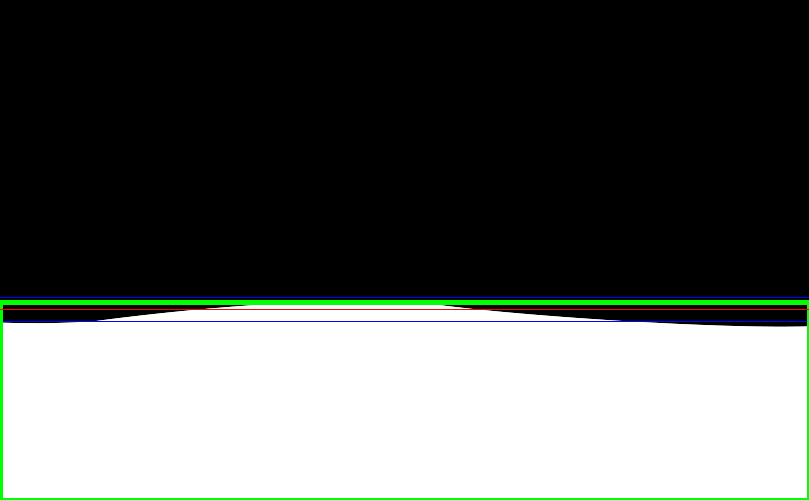
\includegraphics[angle=0,width=0.55\textwidth]{afsnit/afprovning/billeder/naive_losning/naiv_hoisont1.png}
	\end{center}
	\caption{Kun den nederste højrisondt er fundet} 
   	\label{naive_hoisont1}
\end{figure}

\clearpage

\subsection{Afprøvning på malerier}
Vi afprøver den naive algoritme på seks malerier, først på tre malerier,
hvor regions detektoren virker efter vores hensigt og så på ter
malerier, hvor region detektoren ikke virker. Beskrivelsen af hvad der
sker i billedet vil står i caption


\begin{figure}[h!!]
	\begin{center}
		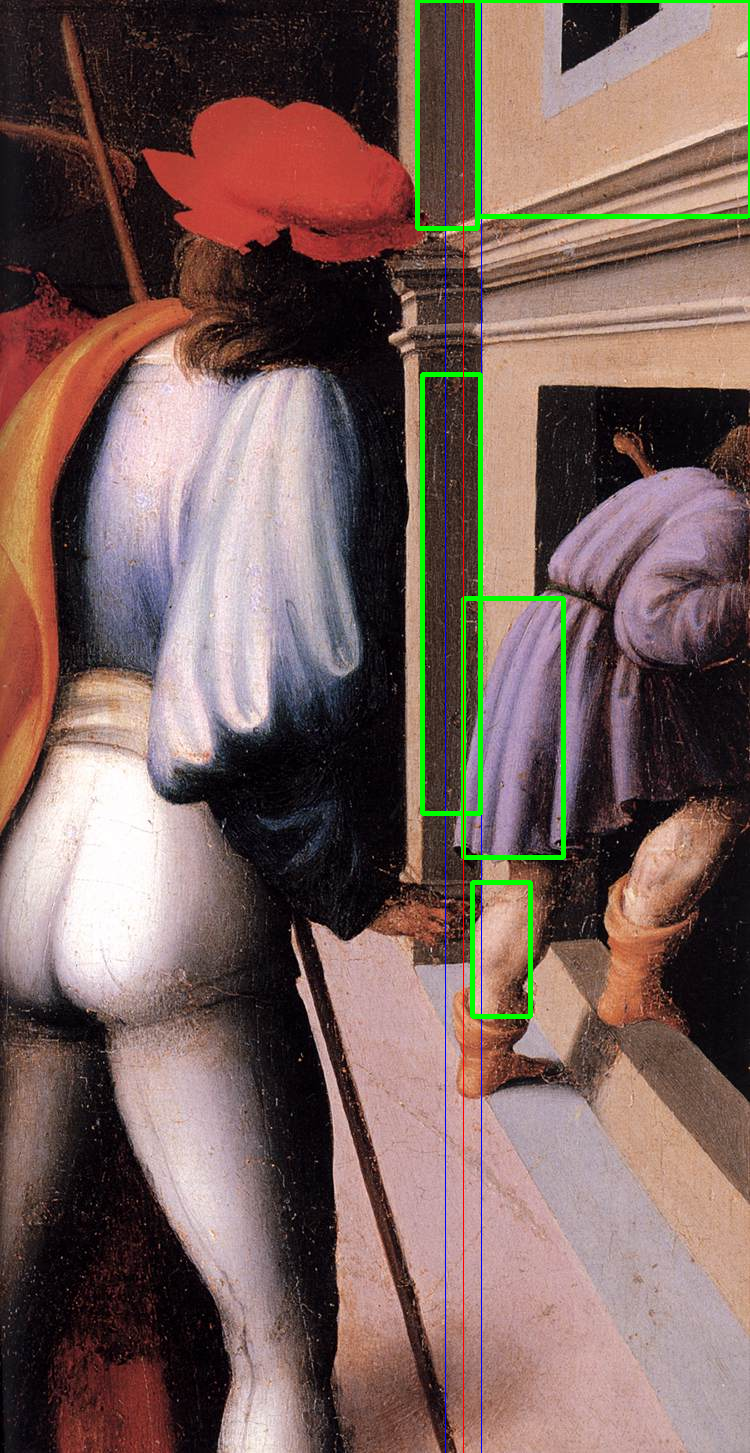
\includegraphics[scale=0.3,angle=0]{afsnit/afprovning/billeder/naive_losning/naiv_kfarver_sdetaljer.png}
	\end{center}
	\caption[]{Fem ud af de seks store regioner fra figur
	\ref{GRD_virker1} valt til at ligge i snittet, skoene er få små til
	at blive taget i betragtning}
	\label{naiv_kfarver_sdetaljer}
\end{figure}

\begin{figure}[h!!]
	\begin{center}
		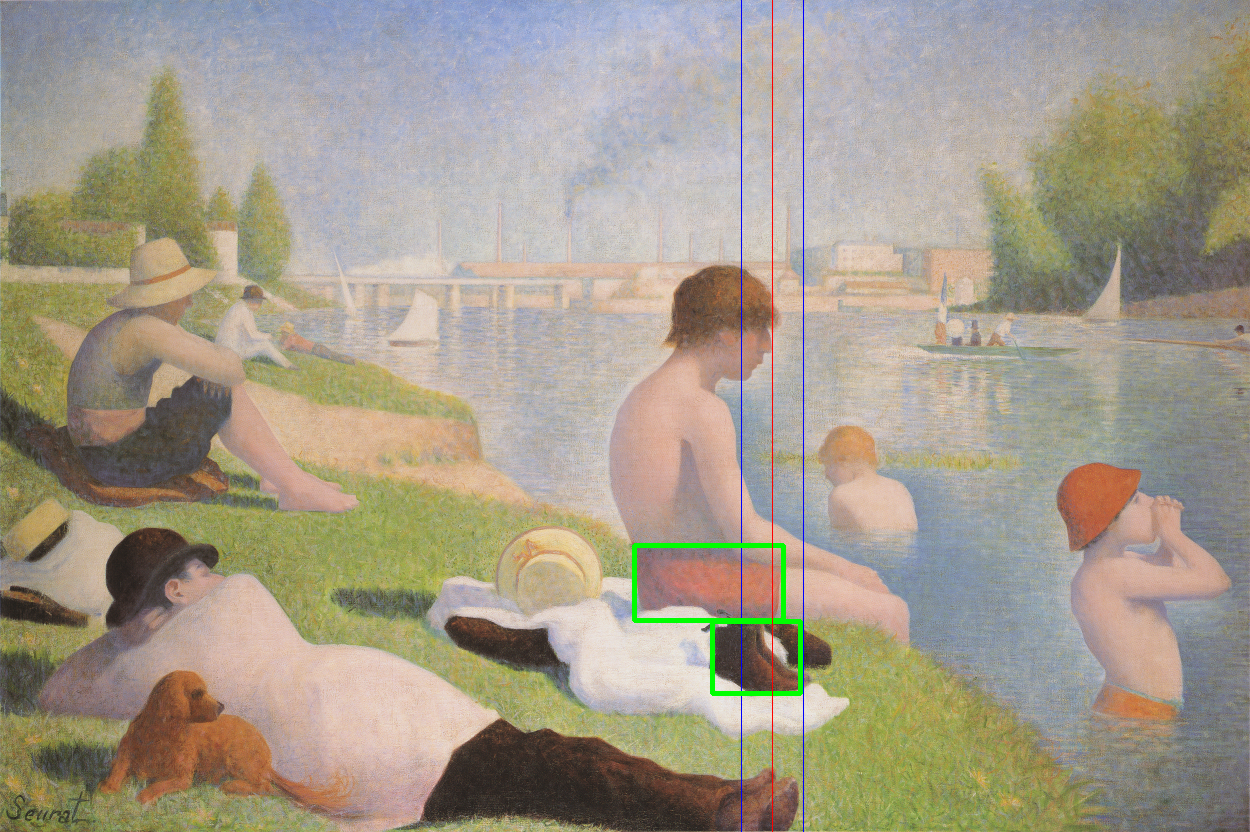
\includegraphics[scale=0.3,angle=0]{afsnit/afprovning/billeder/naive_losning/naiv_mfarver_mdetaljer.png}
	\end{center}
	\caption[]{Bukserne og skoene er tager med af den naive løsning, men
	drengen er sorteret væk da har krydser snittet}
	\label{naiv_mfarver_mdetaljer}
\end{figure}

\begin{figure}[h!!]
	\begin{center}
		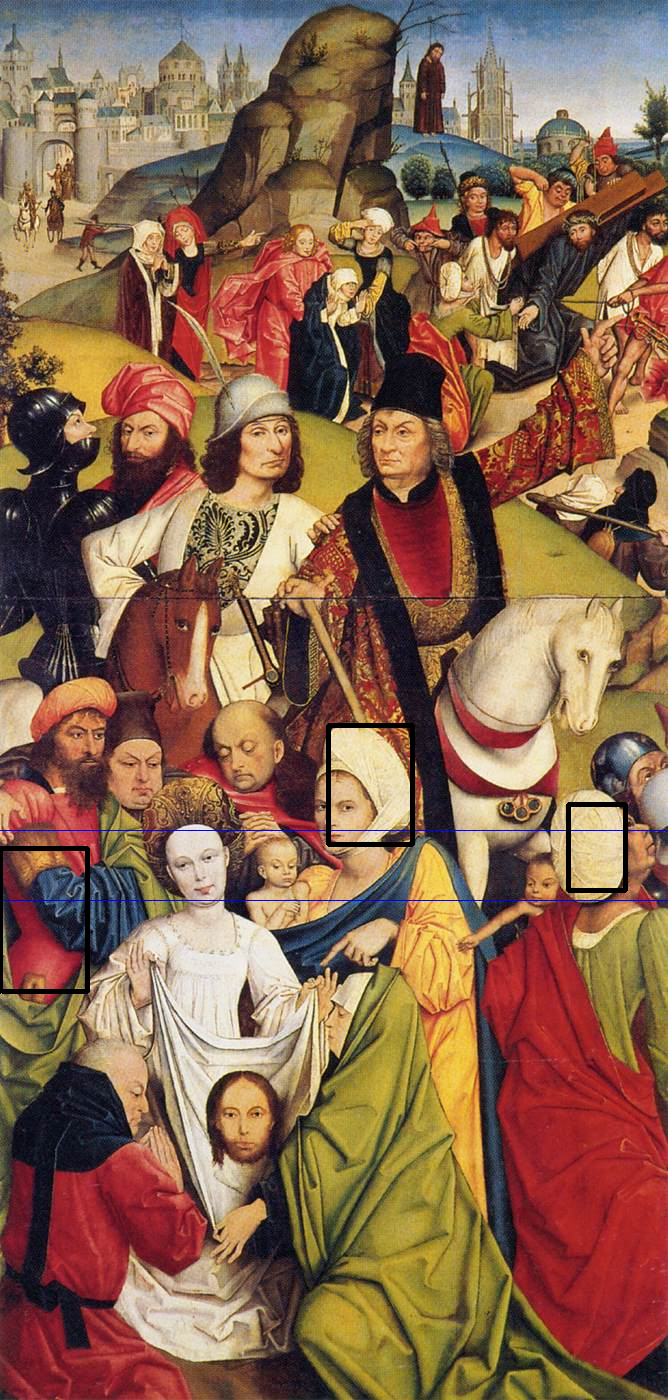
\includegraphics[scale=0.3,angle=0]{afsnit/afprovning/billeder/naive_losning/naiv_kfarver_kdetaljer.png}
	\end{center}
	\caption[]{Et billedet med mange hoder i snittet, hvor to af dem
	bliver godtaget af den naive metode til at ligger i snittet, en
	trøje bliver desværre også taget med. Navn: Christ Carrying the
	Cross. År: 1480. Af: Bosch Hieronymus}
	\label{naiv_kfarver_kdetaljer}
\end{figure}

\begin{figure}[h!!]
	\begin{center}
		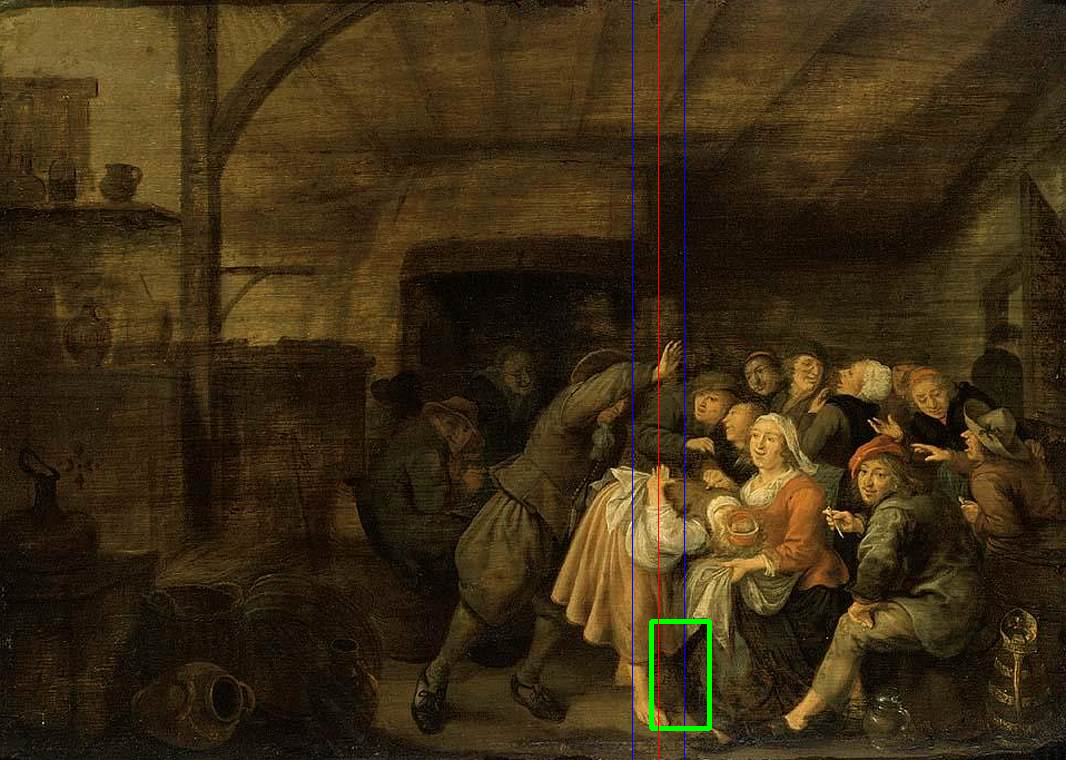
\includegraphics[scale=0.3,angle=0]{afsnit/afprovning/billeder/naive_losning/naiv_virker_ikke1.png}
	\end{center}
	\caption[]{Mallerie hvor region detektor ikke virker, den naive
	løsning godtager tager en region som ligger helt forkert. Navn:
	Peasants in an Inn Playing "La Main Chaude". År: Ukendt. Af:
	Molenaer, Jan Miense.}
	\label{naiv_virker_ikke1}
\end{figure}

\begin{figure}[h!!]
	\begin{center}
		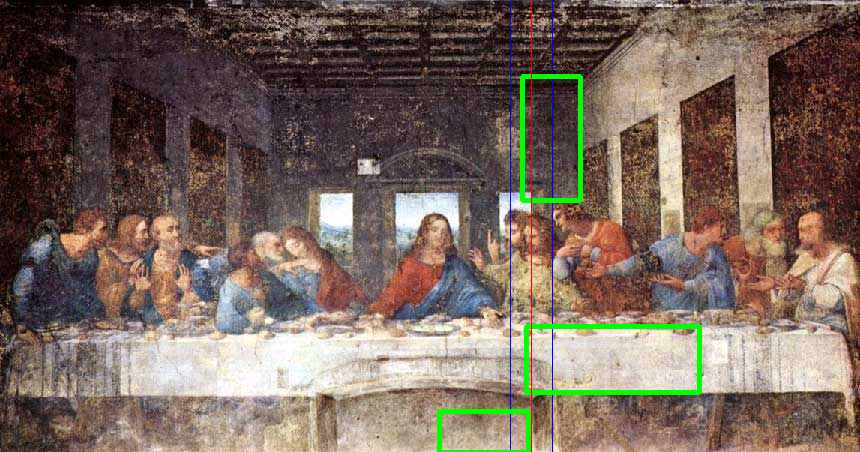
\includegraphics[scale=0.3,angle=0]{afsnit/afprovning/billeder/naive_losning/naiv_virker_ikke2.png}
	\end{center}
	\caption[]{Tre regioner bliver godtaget, selv om de ikke er særlige
	intresante }
	\label{naiv_virker_ikke2}
\end{figure}

\begin{figure}[h!!]
	\begin{center}
		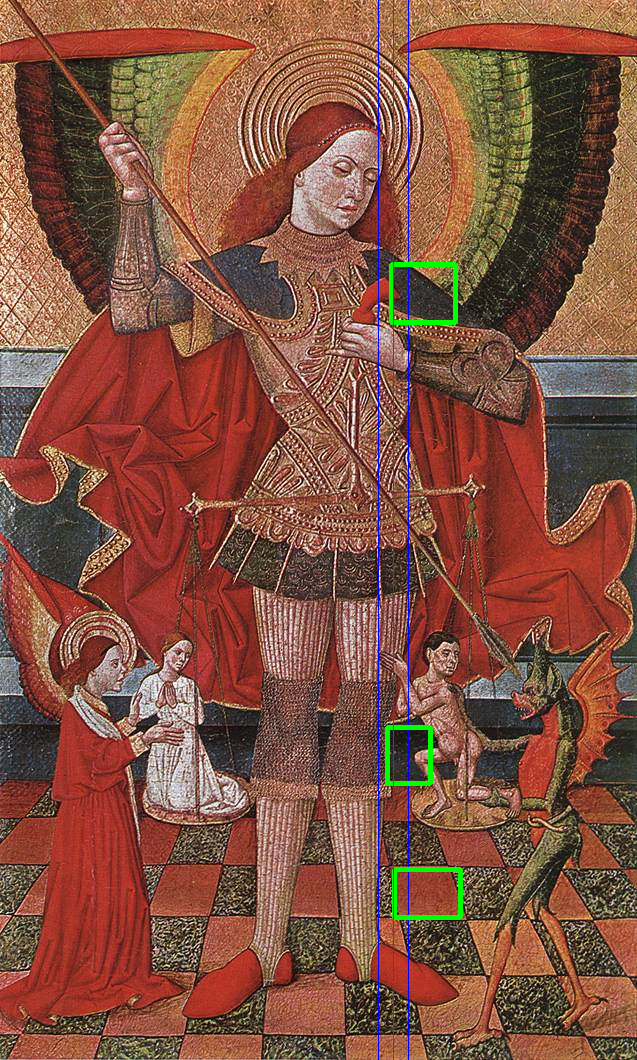
\includegraphics[scale=0.3,angle=0]{afsnit/afprovning/billeder/naive_losning/naiv_virker_ikke3.png}
	\end{center}
	\caption[]{Der bliver fundet tre region, hvor kun en af dem passer
	på en ting i billedet}
	\label{naiv_virker_ikke3}
\end{figure}
\clearpage

\subsection{Konkulution}
Det virker som om den naive løsning virker efter vores entationer dog
med nogle få falske positive, hvis region detektoren virker på
malerierne, dog fejler den på malerier hvor region detektoren fejler, og
kommer med en masse falske positive.

\clearpage

\section{Udvidet løsning}
%% Bemærk:
%%          Resten af rapporten følger en stil hvor indledninger skrives
%%          med \sffamlily-typen. Denne stil bør også følges her.
%%
{\sffamily
I denne sektion vil vi afprøve den udvidede metode for at se, om den
virker efter hensigten på testbilleder og hvordan den virker i praksis
på udvalgte malerier.
}
\subsection{Afprøvning på testbilleder}
Vi afprøver metoden på 4 testbilleder. Billedet \ref{hus_virker} er et hus,
hvor snittet og massemidtpunktet næsten ligger oven i hinanden. 

\begin{figure}[h!!]
	\begin{center}
		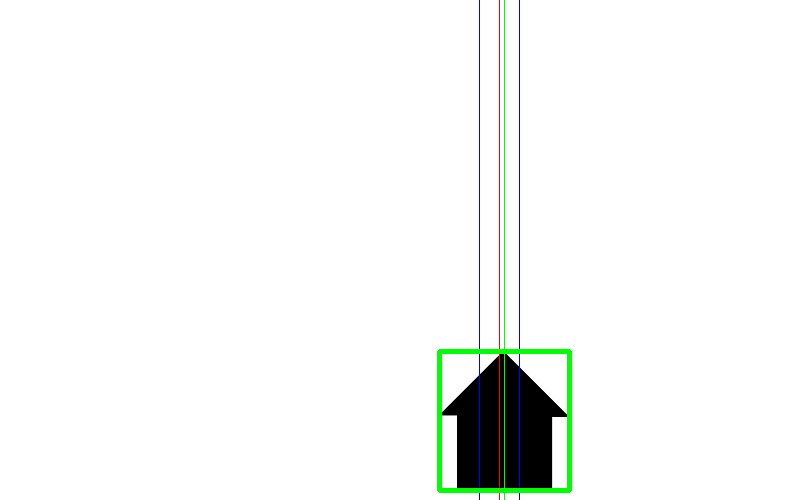
\includegraphics[angle=0,width=0.9\textwidth]{afsnit/afprovning/billeder/udvidet_losning/udvidet_hus1_test.png}
	\end{center}
	\caption[]{Et hus, der er symetrisk og har massemidtpunkt i spisen
	af taget. Massemidtpunktet er inde for margin, så huset bliver
	udvalgt til at ligge i snittet.}
	\label{hus_virker}
\end{figure}

I det andet billede, \ref{hus_virker_ikke}, er huset forskuppet, så massemidtpunktet ligger lige uden for margin, og derved skulle det ikke blive tage
med af metoden. 

\begin{figure}[h!!]
	\begin{center}
		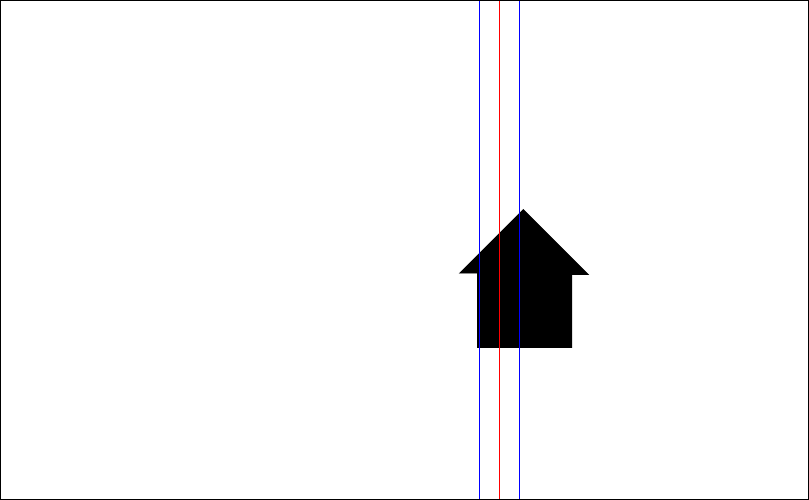
\includegraphics[width=0.9\textwidth,angle=0]{afsnit/afprovning/billeder/udvidet_losning/udvidet_hus2_test.png}
	\end{center}
	\caption[]{Hus, hvor massemidtpunktet er flyttet få pixels uden for margin. Den udvidede metode vælger ikke at tage huset med.}
	\label{hus_virker_ikke}
\end{figure}

Det tredje billedet, \ref{udvidet_blob_test}, har en region, som er
meget lille og derfor bliver sorteret fra. Den store region bliver taget
med, da dens massemidtpunkt ligger inden for margin. 

\begin{figure}[h!!]
	\begin{center}
		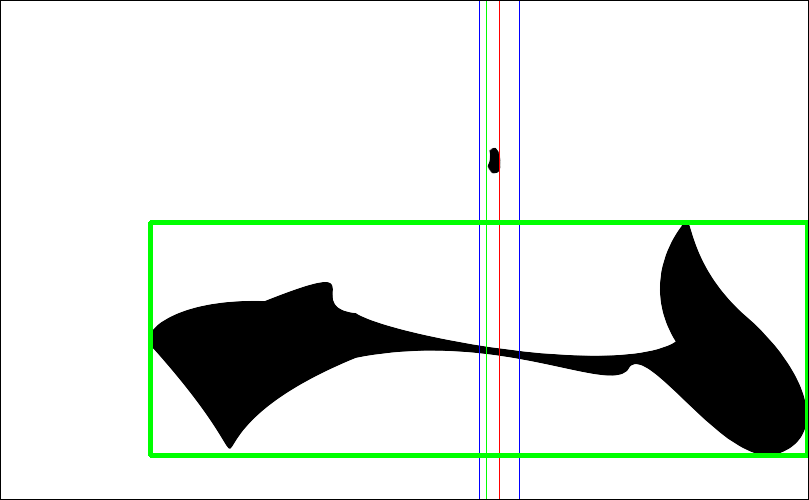
\includegraphics[width=0.9\textwidth,angle=0]{afsnit/afprovning/billeder/udvidet_losning/udvidet_blob2_test.png}
	\end{center}
	\caption[]{To regioner, hvor den nederste har et massemidtpunkt inden for margin.}
	\label{udvidet_blob_test}
\end{figure}

I det fjerde billede, \ref{bleksprutte_test} er der en region, som har
et massemidtpunkt inden for margin, men som har en skæv fordeling af pixels
i forhold til snittet og derfor bliver sorteret fra. Ud fra de fire
observationer, virker det som om, den udvidede metode virker efter
forventningerne.

\begin{figure}[h!!]
	\begin{center}
		\includegraphics[width=0.9\textwidth,angle=0]{afsnit/afprovning/billeder/udvidet_losning/udvidet_bleksprutte_test.png}
	\end{center}
	\caption[]{Margin er sat meget op, så man kan se, at regionen har et massemidtpunkt inden for margin, men da størstedelen af regionens pixels er på højre side, vælges den fra.}
	\label{bleksprutte_test}
\end{figure}

Som man kan se af testbillederne, vælger den udvidedede løsning vidt
forskellige regioner til at ligge i snittet. 
\clearpage


\subsection{Afprøvning på malerier}
Afprøvningen af den udvidede metode på malerier fra vores database
foregår på samme måde som afprøvningen af den naive.

\begin{figure}[h!!]
	\begin{center}
		\includegraphics[width=0.85\textwidth,angle=0]{afsnit/afprovning/billeder/udvidet_losning/udvidet_kfarver_sdetaljer.png}
	\end{center}
	\caption[]{To ud af de seks regioner er godtager som liggende i det gyldne snit af den udvidede metode.}
	\label{udvidet_virker1}
\end{figure}

\begin{figure}[h!!]
	\begin{center}
		\includegraphics[width=0.9\textwidth,angle=0]{afsnit/afprovning/billeder/udvidet_losning/udvidet_dreng.png}
	\end{center}
	\caption[]{Baggrunden er den eneste region som bliver godtaget, da den har et massemidtpunkt, som ligger inden for marginen. Bemærk den grønne kant rundt om hele billedet.}
	\label{udvidet_virker2}
\end{figure}

\begin{figure}[!h]
    \centering
    	\subfloat[Udvidet metode.]{
        	\includegraphics[angle=0,width=0.45\textwidth]{afsnit/afprovning/billeder/udvidet_losning/udvidet_pige.png}
        	\label{udvidet_pige}}\hspace{1em}
    	\subfloat[naiv metode.]{
        	\includegraphics[angle=0,width=0.45\textwidth]{afsnit/afprovning/billeder/udvidet_losning/naiv_pige.png}
        	\label{naiv_pige}}\hspace{1em}        	    			
        \caption[]{Et maleri, hvor resultatet for den udvidede og den naive metode er vist. Der bliver fundet forskellige regioner for hver af metode. Navn: Angel Announcing. År ca. 1500. Af: Bellini, Giovanni.}
     \label{udvidet_virker3}
\end{figure}

\begin{figure}[h!!]
	\begin{center}
		\includegraphics[width=0.9\textwidth,angle=0]{afsnit/afprovning/billeder/udvidet_losning/udvidet_kfarver_kdetaljer.png}
	\end{center}
	\caption[]{En sko og en flise bliver taget med at den udvidede metode.}
	\label{udvidet_virker_ikke1}
\end{figure}

\begin{figure}[h!!]
	\begin{center}
		\includegraphics[width=0.9\textwidth,angle=0]{afsnit/afprovning/billeder/udvidet_losning/udvidet_mfarver_mdetaljer.png}
	\end{center}
	\caption[]{Den udvidede metode sorterer alle regioner væk.}
	\label{udvidet_virker_ikke2}
\end{figure}

\begin{figure}[h!!]
	\begin{center}
		\includegraphics[width=0.9\textwidth,angle=0]{afsnit/afprovning/billeder/udvidet_losning/udvidet_sfarver_mdetaljer.png}
	\end{center}
	\caption[]{To regioner, som ikke repræsenterer noget i billedet, bliver fundet.}
	\label{udvidet_virker_ikke3}
\end{figure}


Ud fra tabellerne \ref{udvidet_good} og \ref{udvidet_bad}, hvor de
interressante og falske positiver er opstillet --- som i den naive
afprøvning --- kan det ses, at der blive fundet 7 interessante regioner og 5
falske positiver. Det vil sige 40 \% flere interessante regioner en falske
positiver.

\begin{table}[H]
    \centering
    \begin{tabular}{|c|l|l|l|}
	\hline
           				& Kraftige farver & Medium farver & Svage farver \\\hline
		Mange detaljer	& 1 & 0 & 1 \\\hline
        Medium detaljer & 0 & 1 & 0 \\\hline
        Få detaljer     & 0 & 0 & 4 \\\hline
    \end{tabular}
    \caption[]{Tabel over antal interessante regioner i det gyldne snit 0 i ni test malerier.}
    \label{udvidet_good}
\end{table}

\begin{table}[H]
    \centering
    \begin{tabular}{|c|l|l|l|}
		\hline
            & Kraftige farver & Medium farver & Svage farver \\\hline
		Mange detaljer	& 0 & 2 & 1 \\\hline
        Medium detaljer  & 0 & 3 & 0 \\\hline
        Få detaljer     & 2 & 3 & 0 \\\hline
    \end{tabular}
    \caption[]{Tabel over antal falske positiver i det gyldne snit 0 i ni test malerier.}
    \label{udvidet_bad}
\end{table}
\clearpage

\subsection{Konklusion}
Den udvidede metode virker som vi havde planlagt på de ensfarvede
regioner i testbillederne I praksis er den udvidede metode merer
effektiv end den naive: Som man kan se i figur \ref{udvidet_virker3} finder
den $20 \%$ flerer interessante regioner end falske positiver, end den
naive metode gør. Selv om den udvidede stadig kun finder $40\%$ flere
interessante regioner en falske positiver, er det ikke helt dårligt, i
betratning af, at vores regiondetektor ikke virker optimalt. Alt i alt
er det alså en god løsning.

\clearpage

\section{Sammelining af de 2 metoder?}
Ud for de 2 metoders konklution laver vi en sammenligning af de 2 metoder. Den første metode finder mange gode regioner, men også mange ikke så gode regioner, Den anden metode finder en del fære gode regioner, men meget få ikke så gode regioner
den her vil jeg have hjælp til






\clearpage


}

% vim: set tw=72 spell spelllang=da:
